\section{Визуализация квантовой части релятивистского протокола распределения ключей}
Программа, визуализирующая процесс квантовой части протокола, была названа Requc (от Relativistic Quantum Cryptography) и в дальнейшем при необходимости будет использоваться именно это название.
Исходя из схемы протокола, в программе имеется две основных модели - модель квантового состояния и модель единичной посылки. 

Диаграмма классов представлена на рисунке \ref{fig:requc_models}
\begin{figure}[h]
  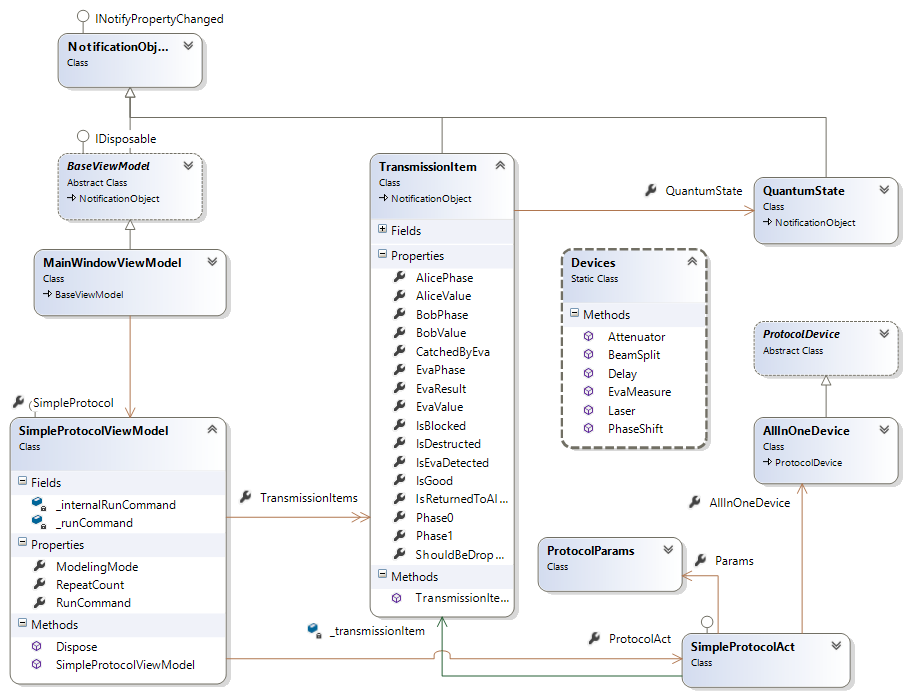
\includegraphics[width=0.9\linewidth]{chapter3/requc_models}
  \caption{Диаграмма классов программы Requc.}
  \label{fig:requc_models}
\end{figure}

Согласно описанному выше шаблону MVVM, все классы, имена которых оканчиваются на \textit{ViewModel}, являются Моделями Представлениями. 
В силу относительной визуальной простоты программы (нет сложной логики интерфейса, множества экранов и т.п.), по факту на протяжении всего жизненного цикла программы используется лишь одна модель представления~--- \mintinline{csharp}|SimpleProtocolViewModel|. Эта модель представления содержит ссылку на коллекцию объектов Модели \mintinline{csharp}|TransmissionItem|, представляющей собой объект посылки в протоколе, и ссылку на экземпляр Модели \mintinline{csharp}|SimpleProtocolAct|, который содержит метод (на схеме не указан) запуска очередной итерации протокола по описанной в пункте \ref{sec:common_description} схеме.

Главный экран программы показан на рисунке \ref{fig:requc_start_state}. В верхней части экрана по центру изображен оптический тракт между Алисой и Бобом с подслушивателем Евой в середине. В нижней части по центру изображена пространственно-временная плоскость. Слева от нее таблица с результатами каждого прохода. Справа вверху управляющие графические элементы, задающие режим моделирования, число повторений и запуск визуализации.

Данный экран отрисовывается Представлением \mintinline{csharp}|SimpleProtocolView|. Иерархия Представлений изображена на рисунке \ref{fig:requc_views}. Так как Представления не производят никаких действий над данными, а только отображают их, то жесткими связями, которые можно было бы изобразить на диаграмме классов, они не обладают, так как в принципе не содержат ссылок на экземпляры других Представлений или Модели представлений. Связывание данных происходит во время исполнения программы, и всю заботу об этом на себя берет WPF.
\begin{figure}[h]
  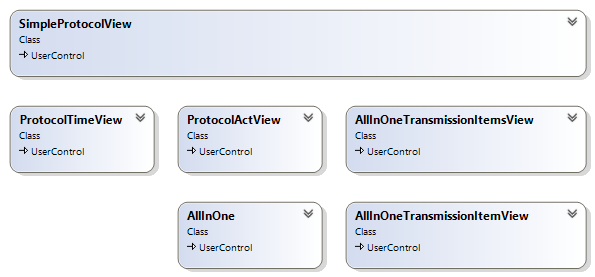
\includegraphics[width=0.9\linewidth]{chapter3/requc_views}
  \caption{Иерархия Представлений программы Requc.}
  \label{fig:requc_views}
\end{figure}

После задания необходимых параметров пользователь нажимает кнопку и запускает процесс моделирования, который тут же наглядно визуализируется. 
Вкратце, это работает следующим образом:
\begin{itemize}
  \item Обработчик события \mintinline{csharp}{Cliked} кнопки запускает команду \mintinline{csharp}{RunCommand} на выполнение.
  \item В методе \mintinline{csharp}{Execute} экземпляра команды происходит выполнение кода, запускающего внутреннюю логику моделирования:
    \begin{csharpcode}
      var item = _protocolAct.Process(_modelingMode);
      _transmissionItems.Add(item);
    \end{csharpcode}
  \item В методе \mintinline{csharp}{SimpleProtocolAct.Process} происходит создание экземпляра посылки и квантового состояний, моделирование их преобразований и передачи по каналу связи. По окончанию каждого этапа (проход от Алисы до Боба и обратный проход от Боба до Алисы) вызываются соответствующие события \mintinline{csharp}{Started} и \mintinline{csharp}{Finished}. Наступления этих событий ожидают все Представления, чтобы начать визуализацию по актуальным данным.
\end{itemize}

В программе Requc сначала полностью просчитывается результат моделирования, который затем визуализируется. Это позволяет несколько упростить код и уменьшить число необходимых классов. В другой программе, Cascade (см. далее) такой подход не применим, так как существует зависимость одних шагов от результатов работы других. Как это было решено, описано в соответствующем разделе.

Далее представлены снимки экрана программы в различные моменты выполнения. Исходный код доступен в приложении \ref{app:requc}.
\begin{figure}[h]
  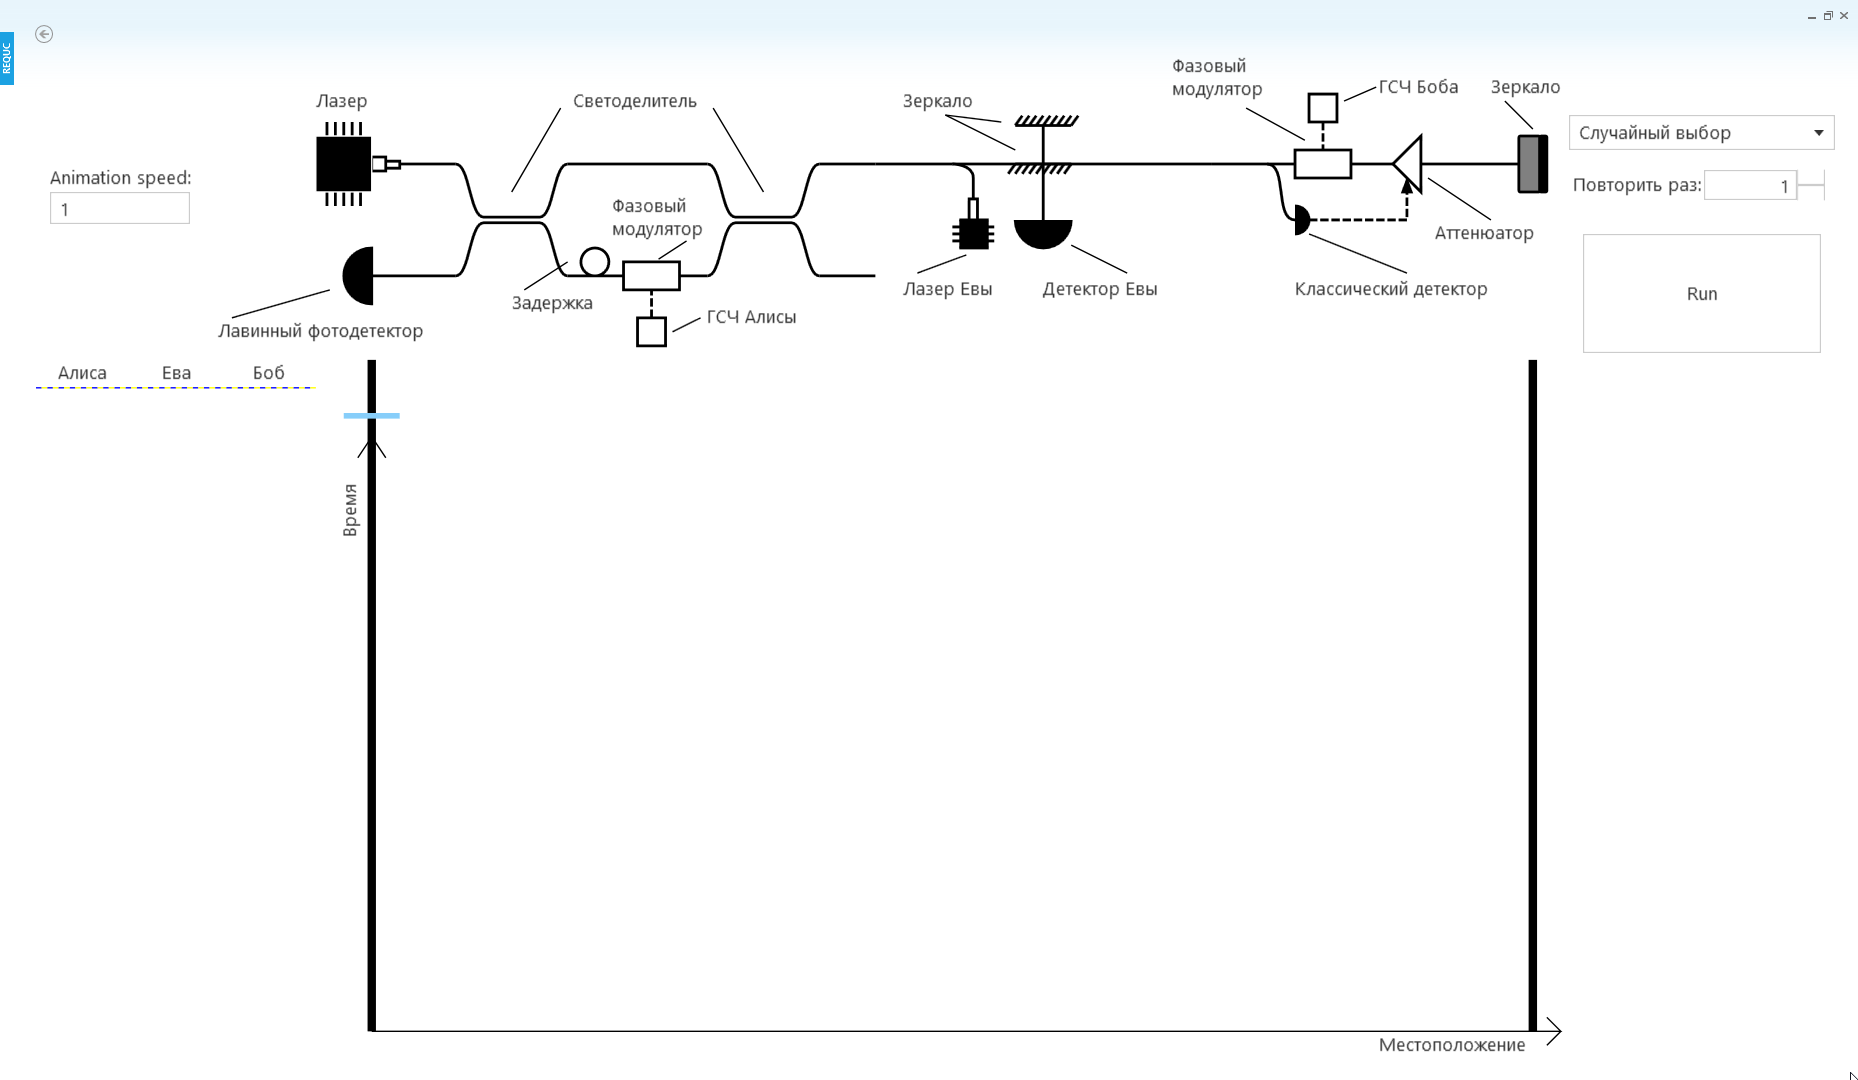
\includegraphics[width=0.9\linewidth]{chapter3/requc_start_state}
  \caption{Начальное состояние программы Requc.}
  \label{fig:requc_start_state}
\end{figure}

\begin{figure}[h]
  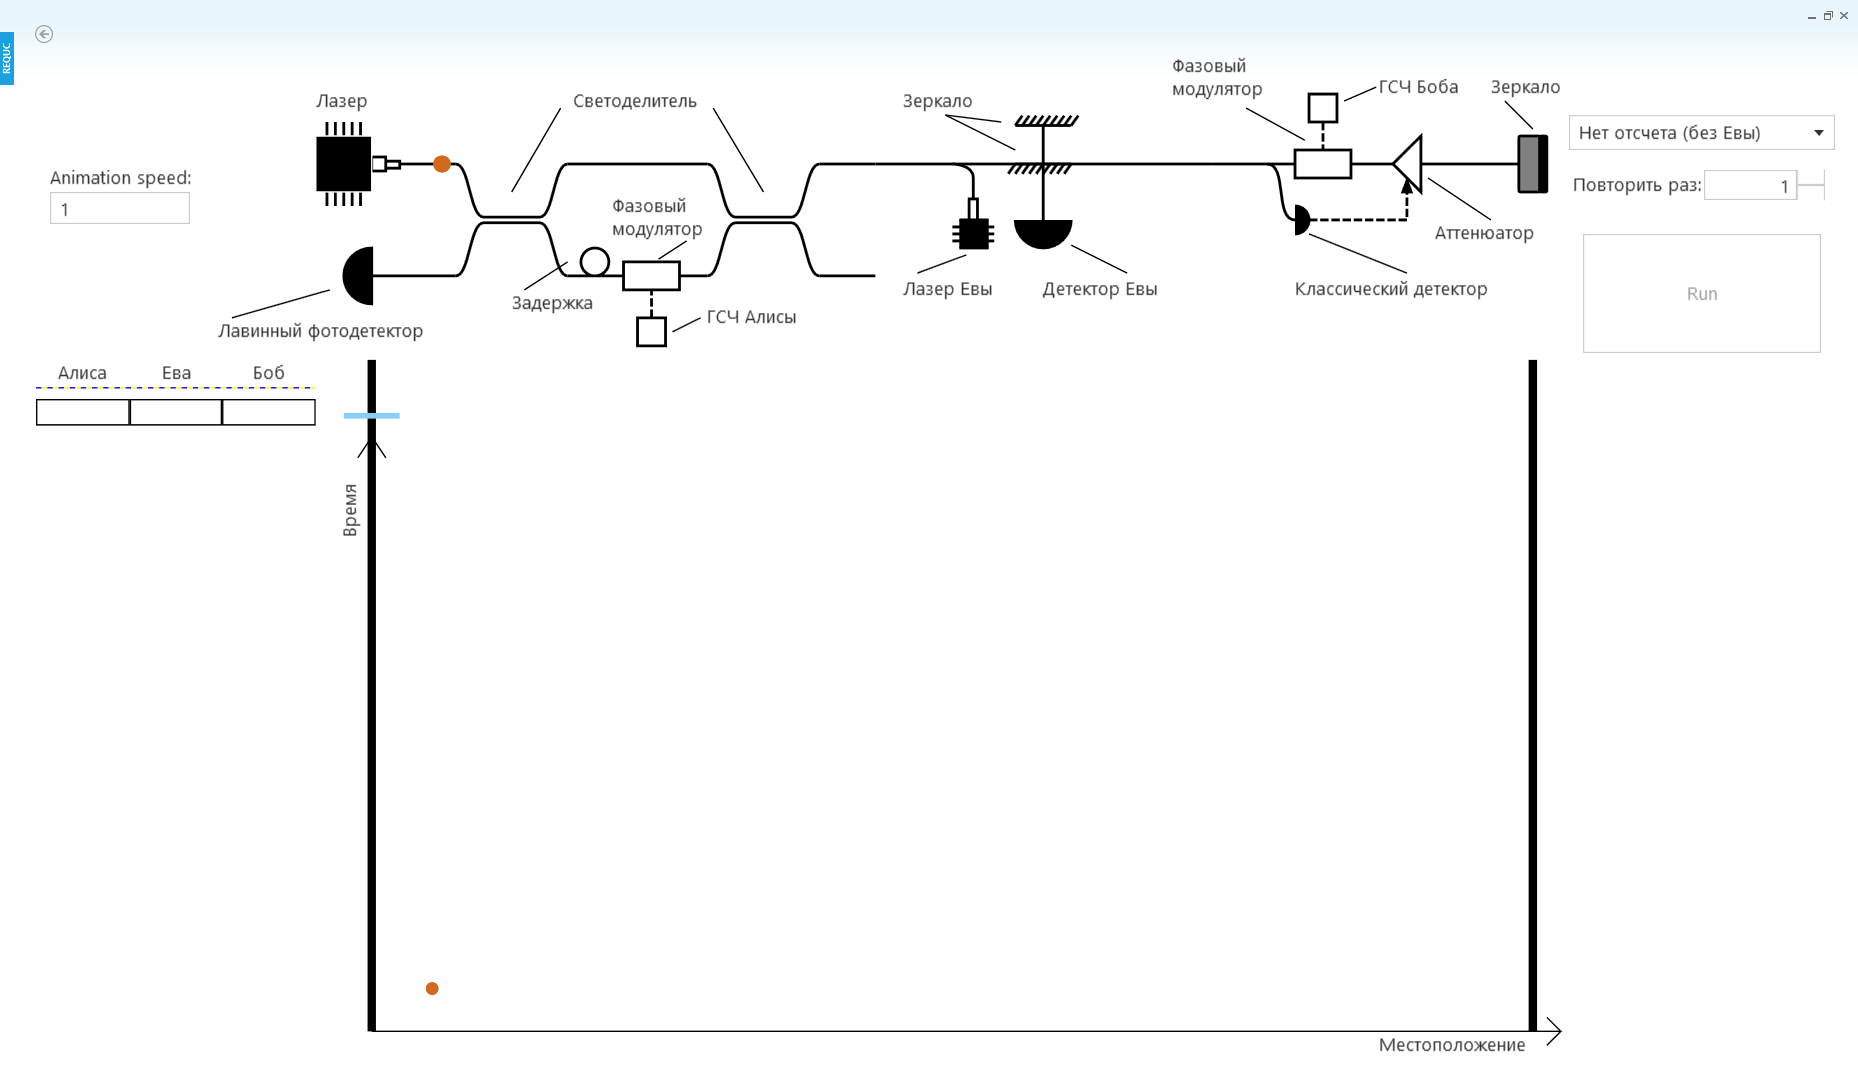
\includegraphics[width=0.9\linewidth]{chapter3/requc_screenshots/01_laser}
  \caption{Алиса испускает классическое когерентное состояние.}
\end{figure}

\begin{figure}[h]
  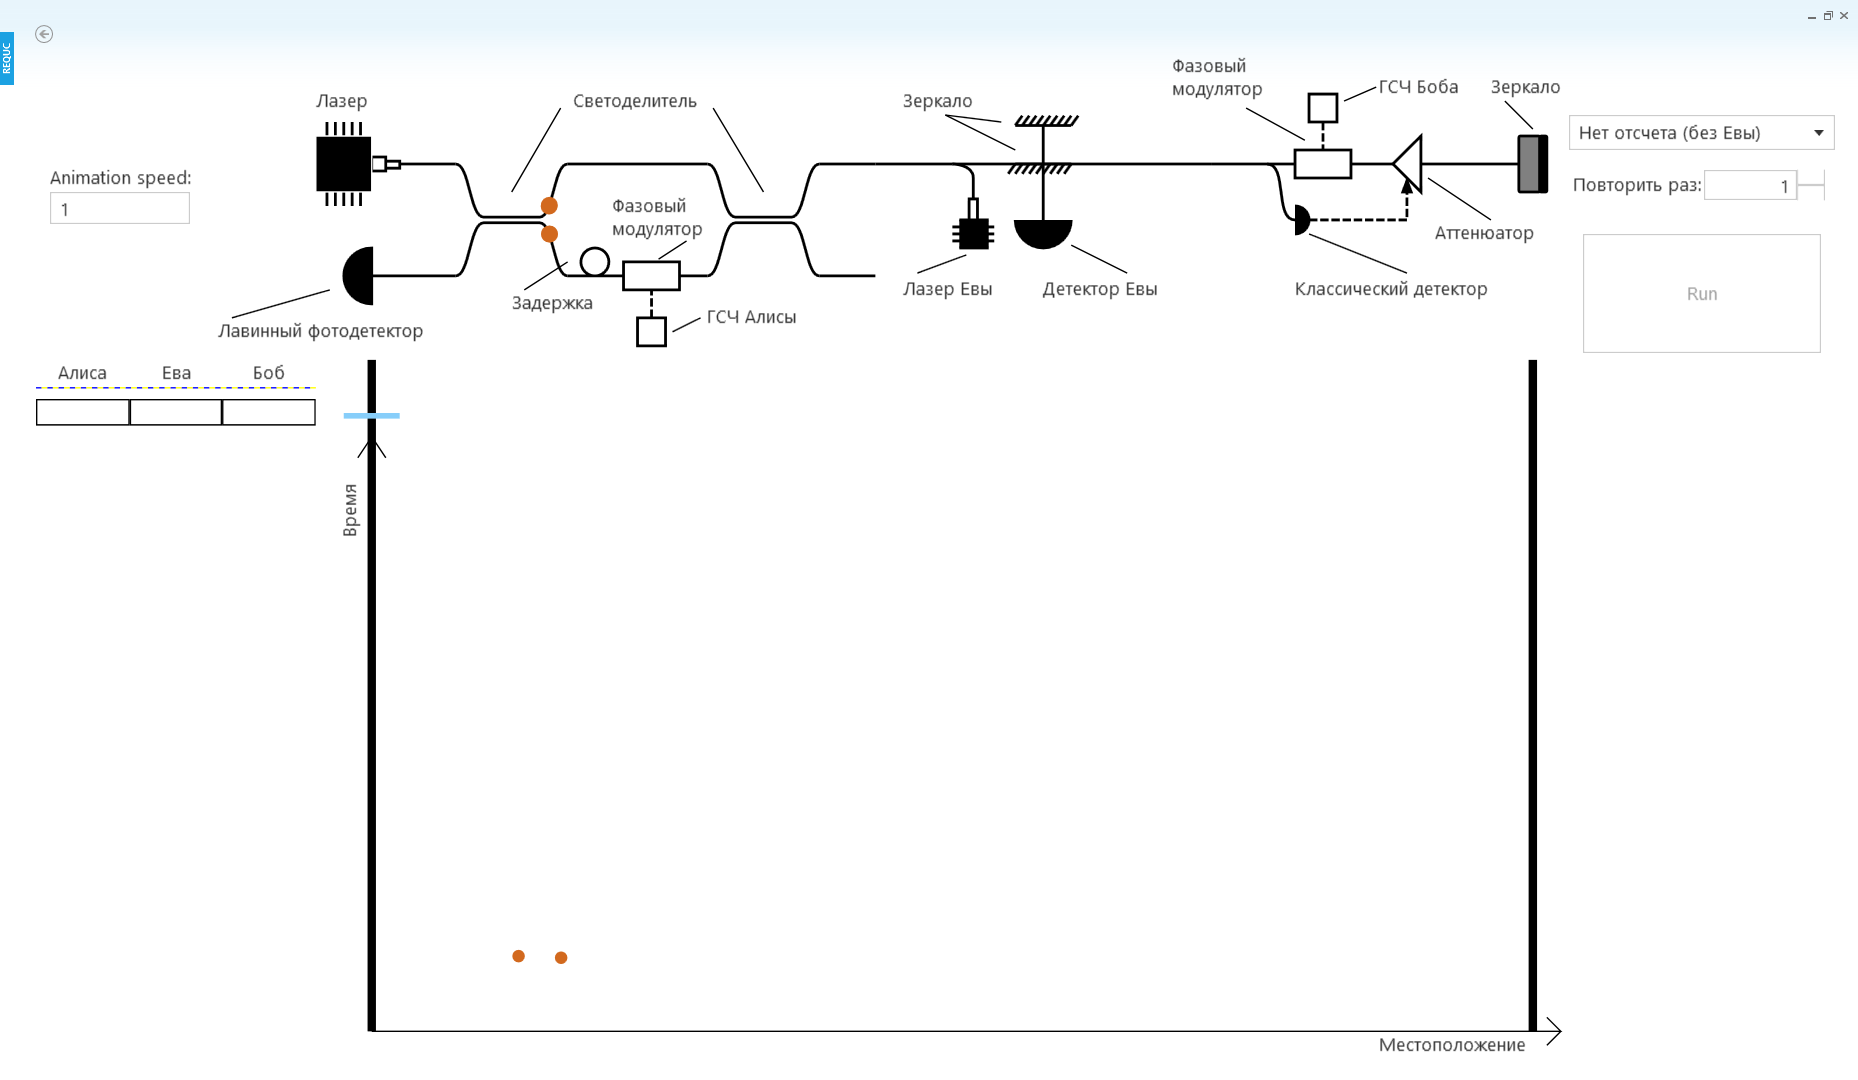
\includegraphics[width=0.9\linewidth]{chapter3/requc_screenshots/02_beam}
  \caption{Преобразование состояния на светоделителе.}
\end{figure}

\begin{figure}[h]
  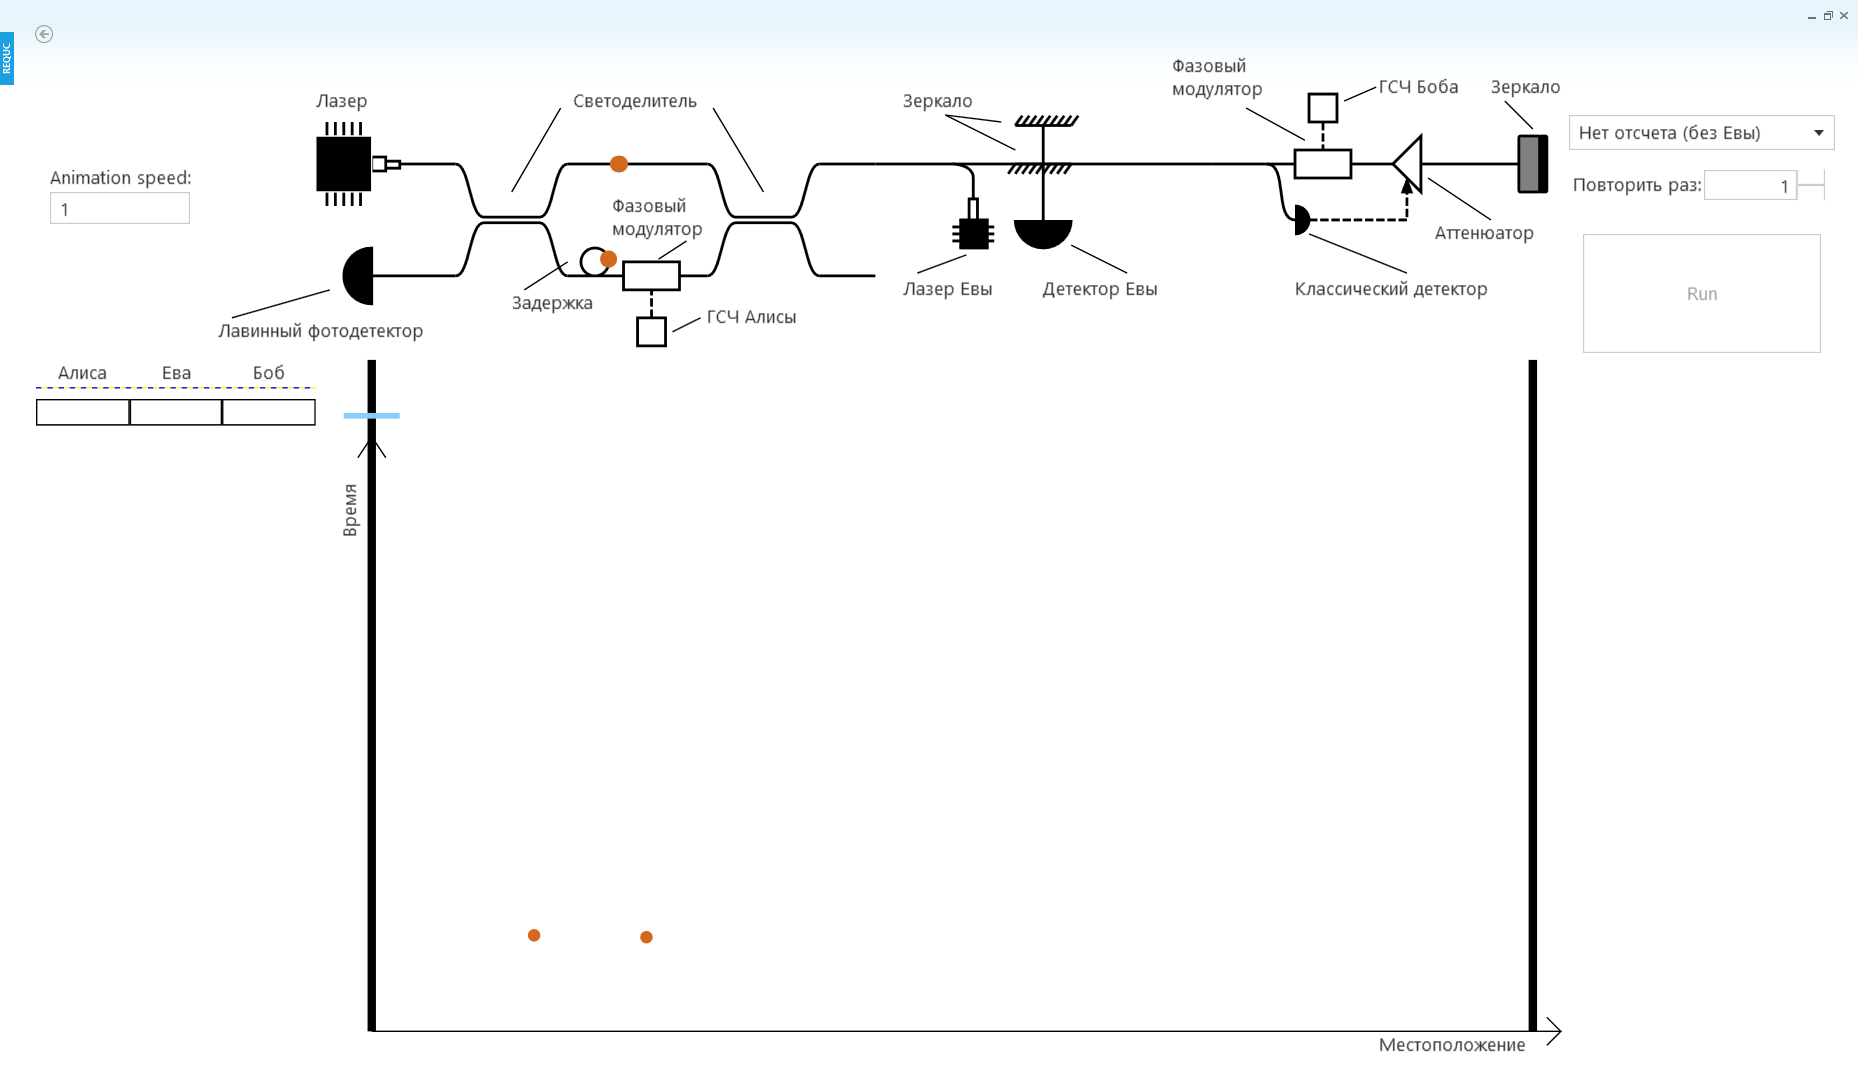
\includegraphics[width=0.9\linewidth]{chapter3/requc_screenshots/03_delay}
  \caption{Задержка нижней половинки состояния~--- разнесение половинок в пространстве (см. нижнюю часть экрана).}
\end{figure}

\begin{figure}[h]
  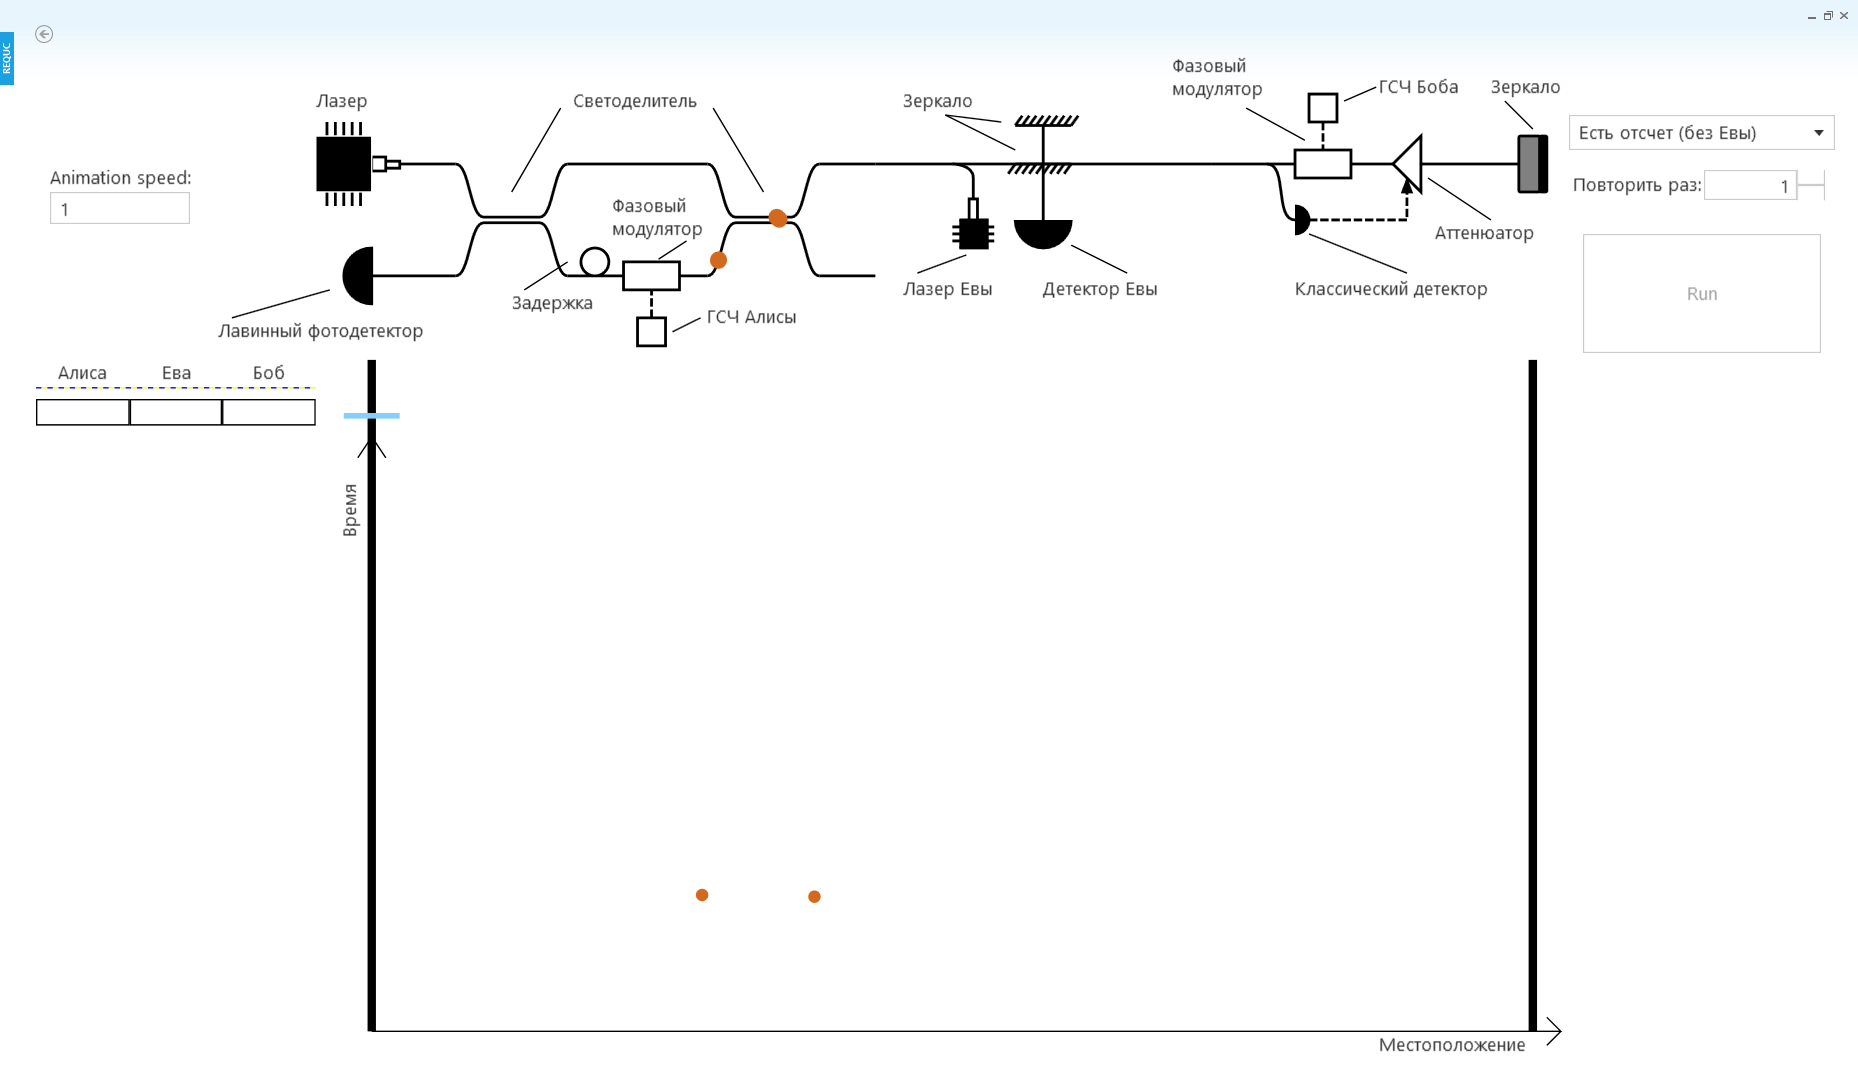
\includegraphics[width=0.9\linewidth]{chapter3/requc_screenshots/04_beam2}
  \caption{Преобразование <<растянутого>> состояния на светоделителе.}
\end{figure}

\begin{figure}[h]
  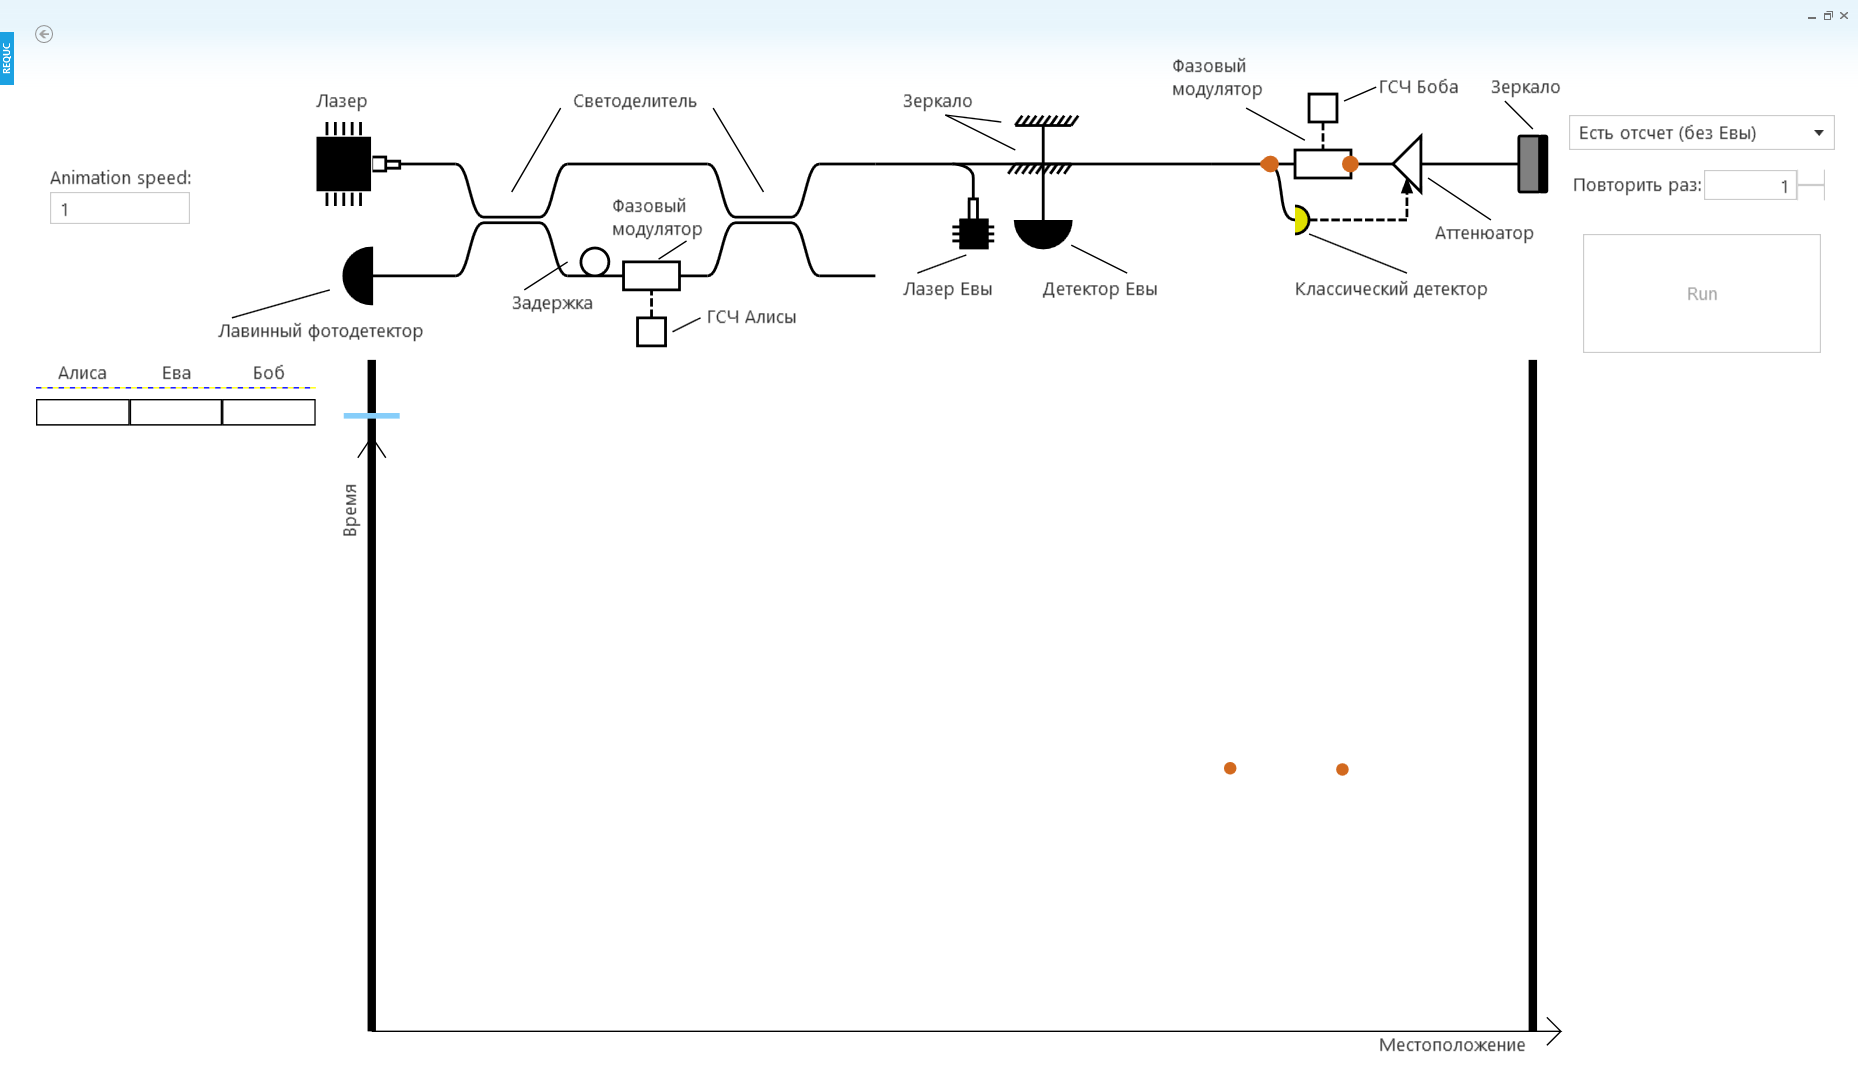
\includegraphics[width=0.9\linewidth]{chapter3/requc_screenshots/07_bob_detector}
  \caption{Срабатывание детектора Боба, отмечающего время прихода состояния.}
\end{figure}

\FloatBarrier

\begin{figure}[h]
  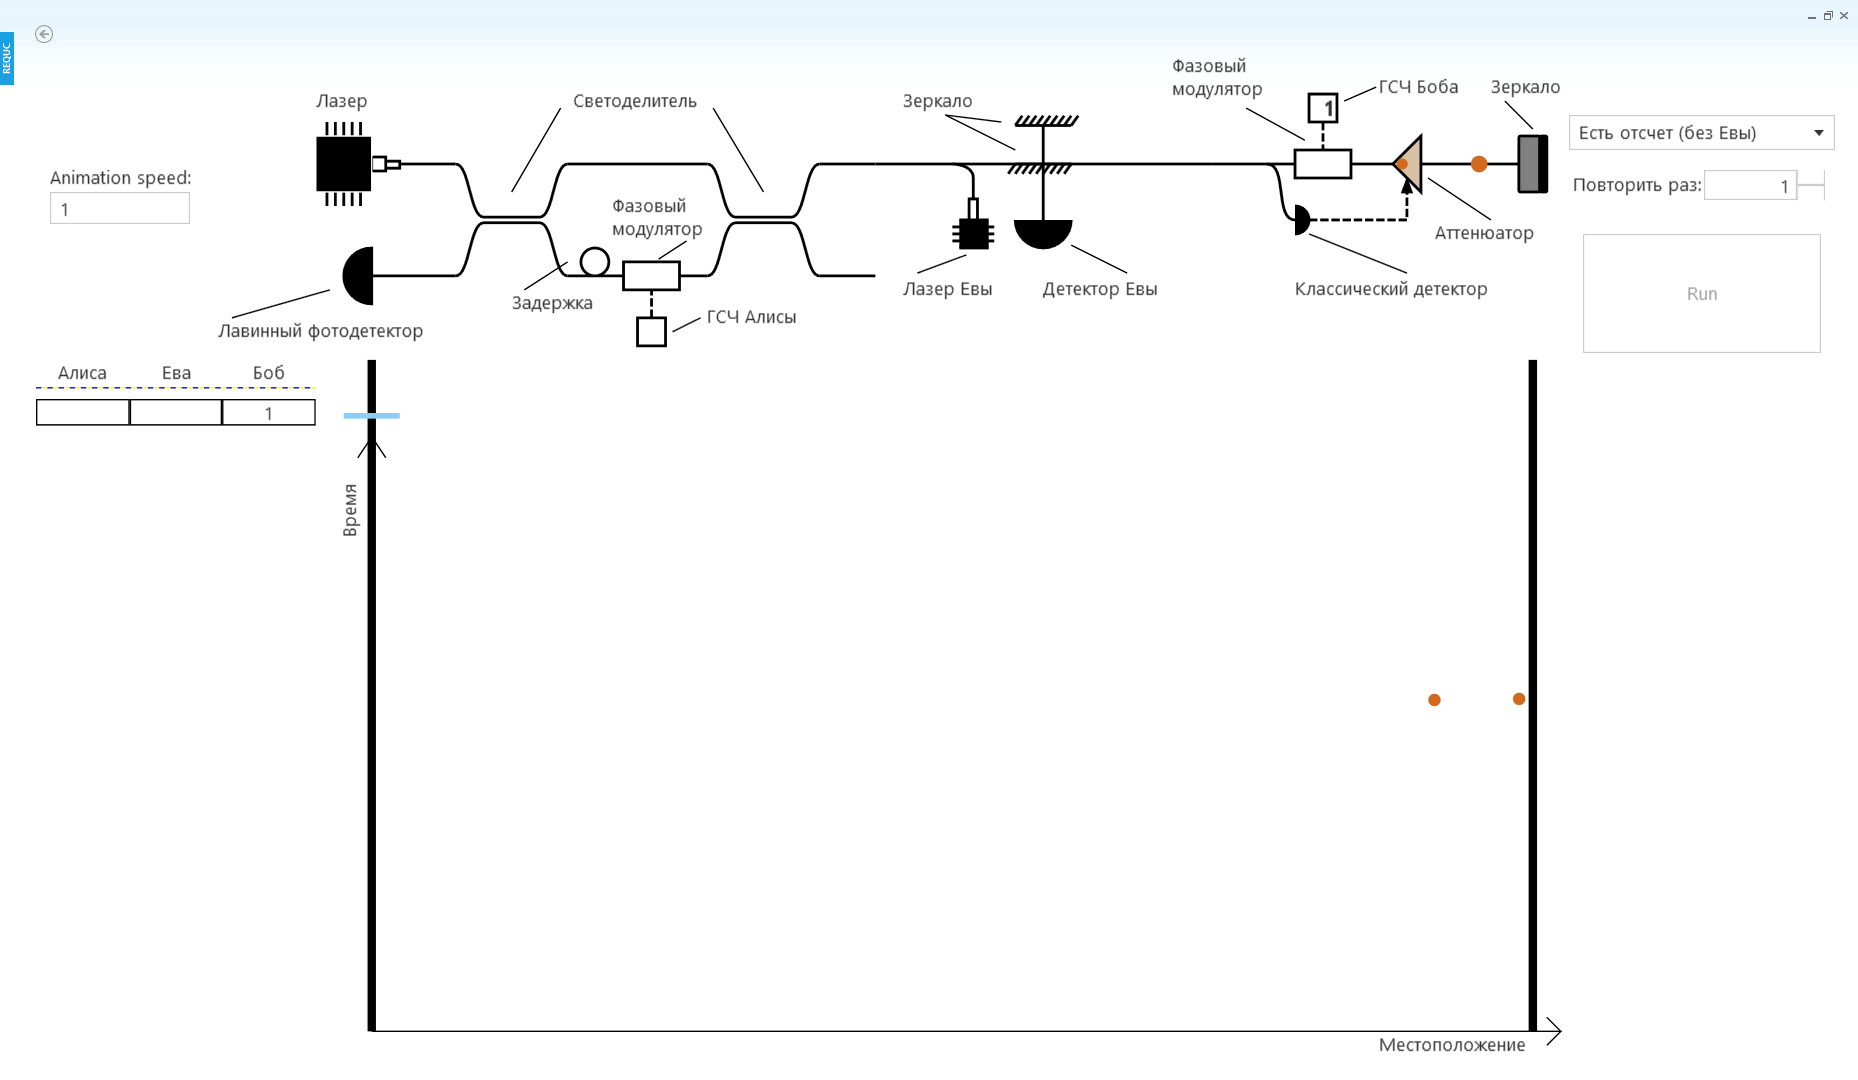
\includegraphics[width=0.9\linewidth]{chapter3/requc_screenshots/08_bob_attenuator}
  \caption{Ослабление сигнала до квазиоднофотонного уровня.}
\end{figure}

\begin{figure}[h]
  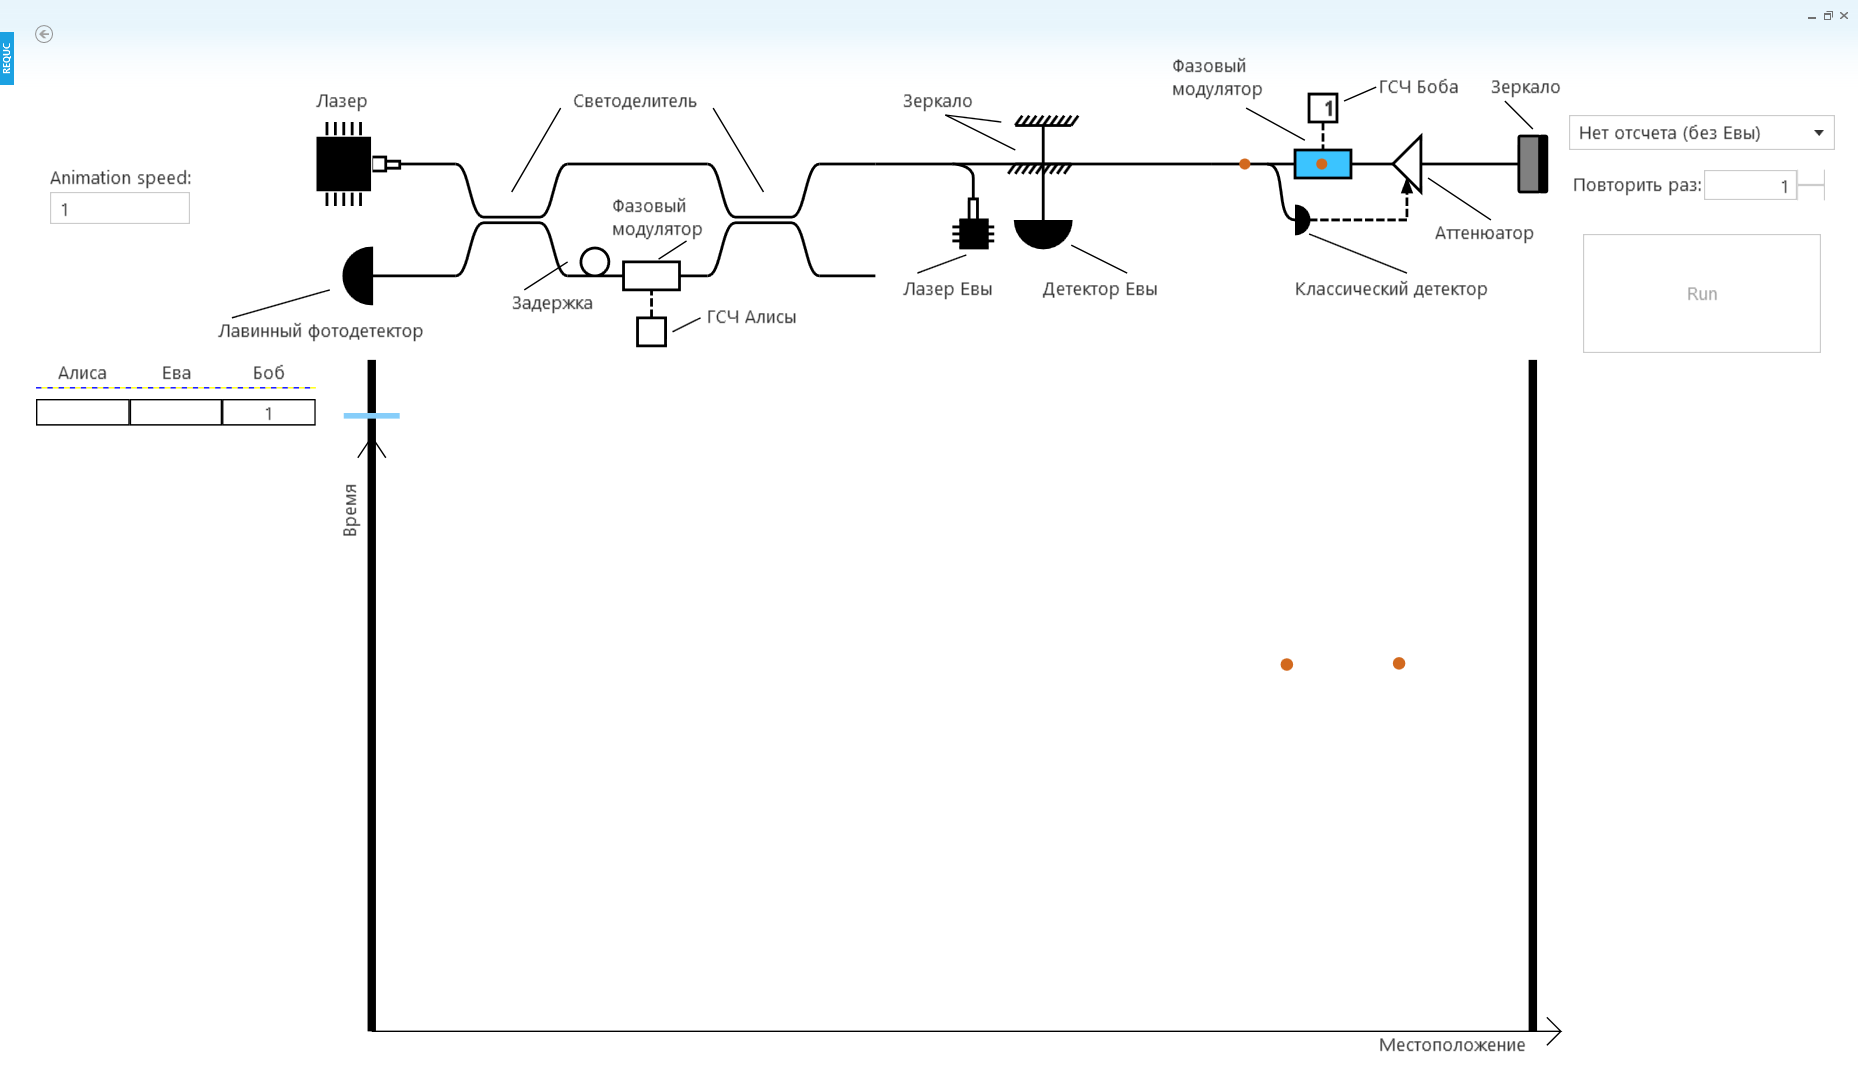
\includegraphics[width=0.9\linewidth]{chapter3/requc_screenshots/09_bob_phase}
  \caption{Применение фазового модулятора со случайно выбранной из двух вариантов фазой к половинке состояния, локализованной во втором временном окне.}
\end{figure}

\begin{figure}[h]
  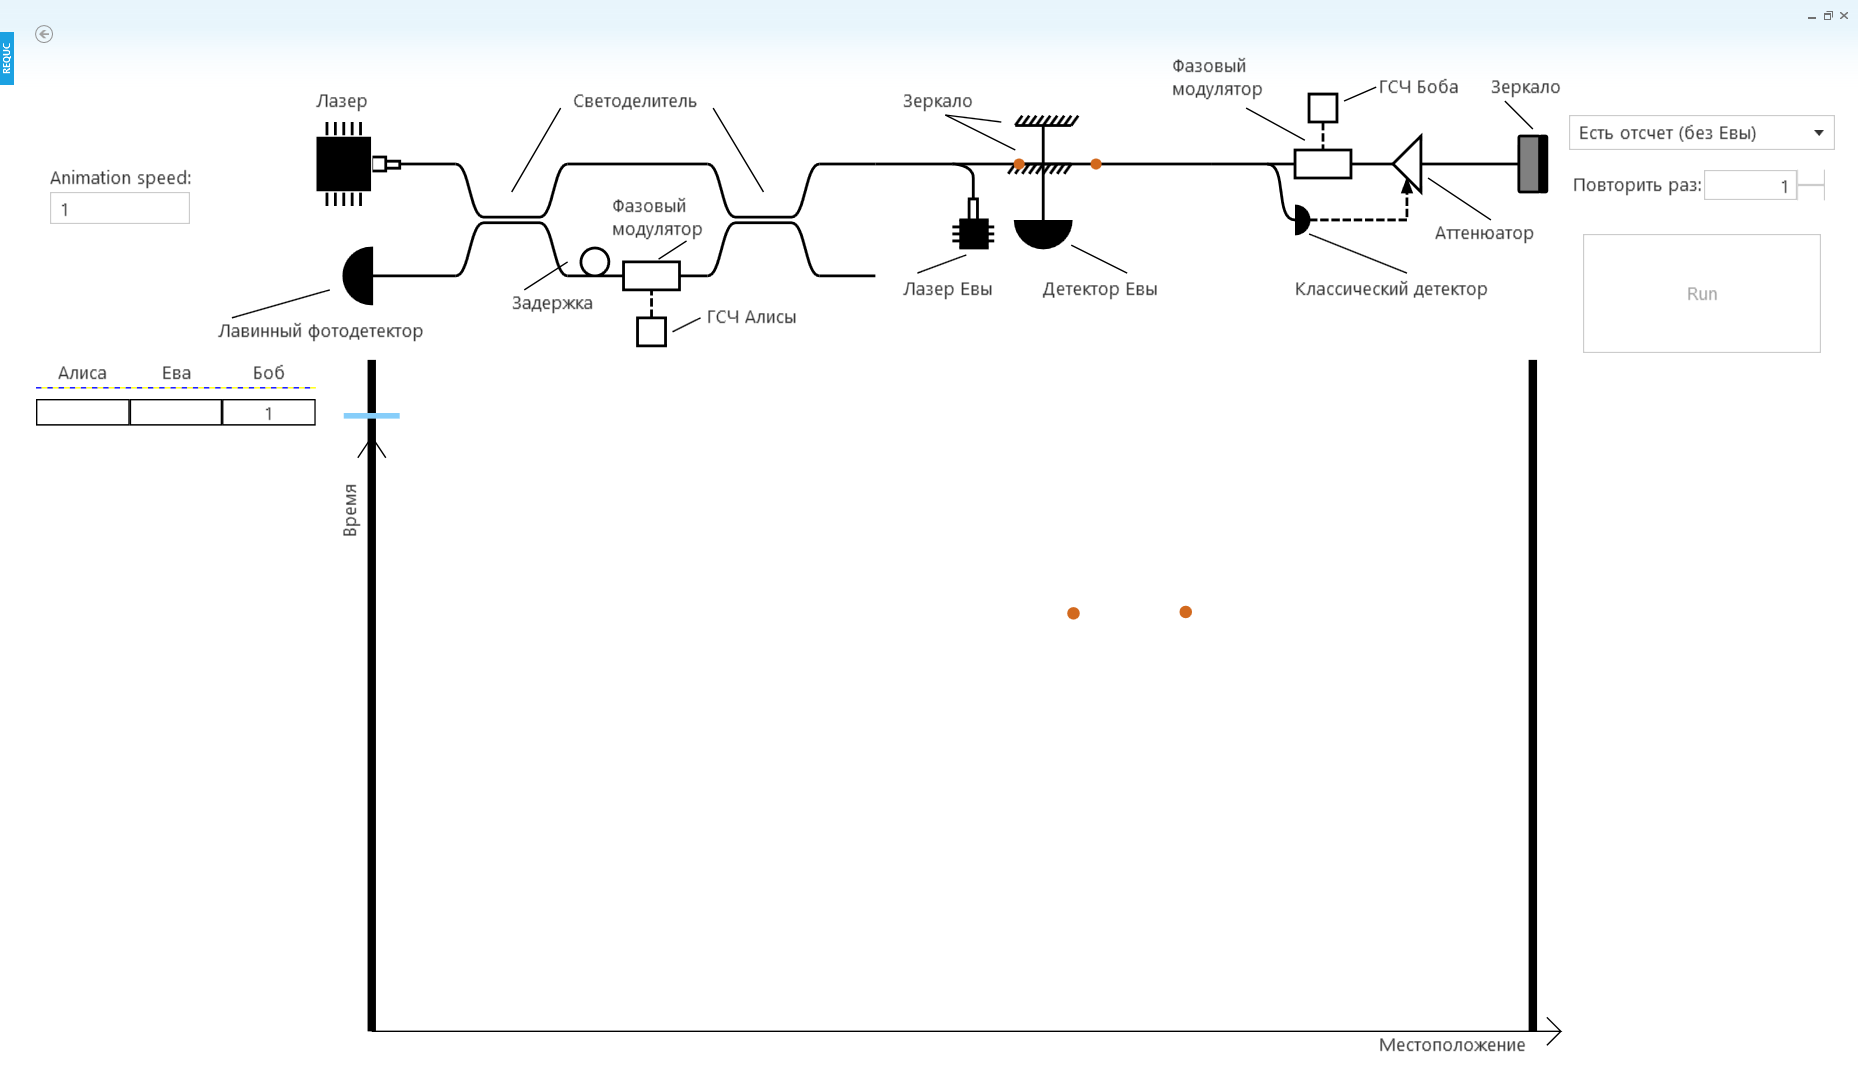
\includegraphics[width=0.9\linewidth]{chapter3/requc_screenshots/10_eva_pass}
  \caption{Ева не перехватывает посылку и не получает никакой информации о соответствующем бите.}
\end{figure}

\begin{figure}[h]
  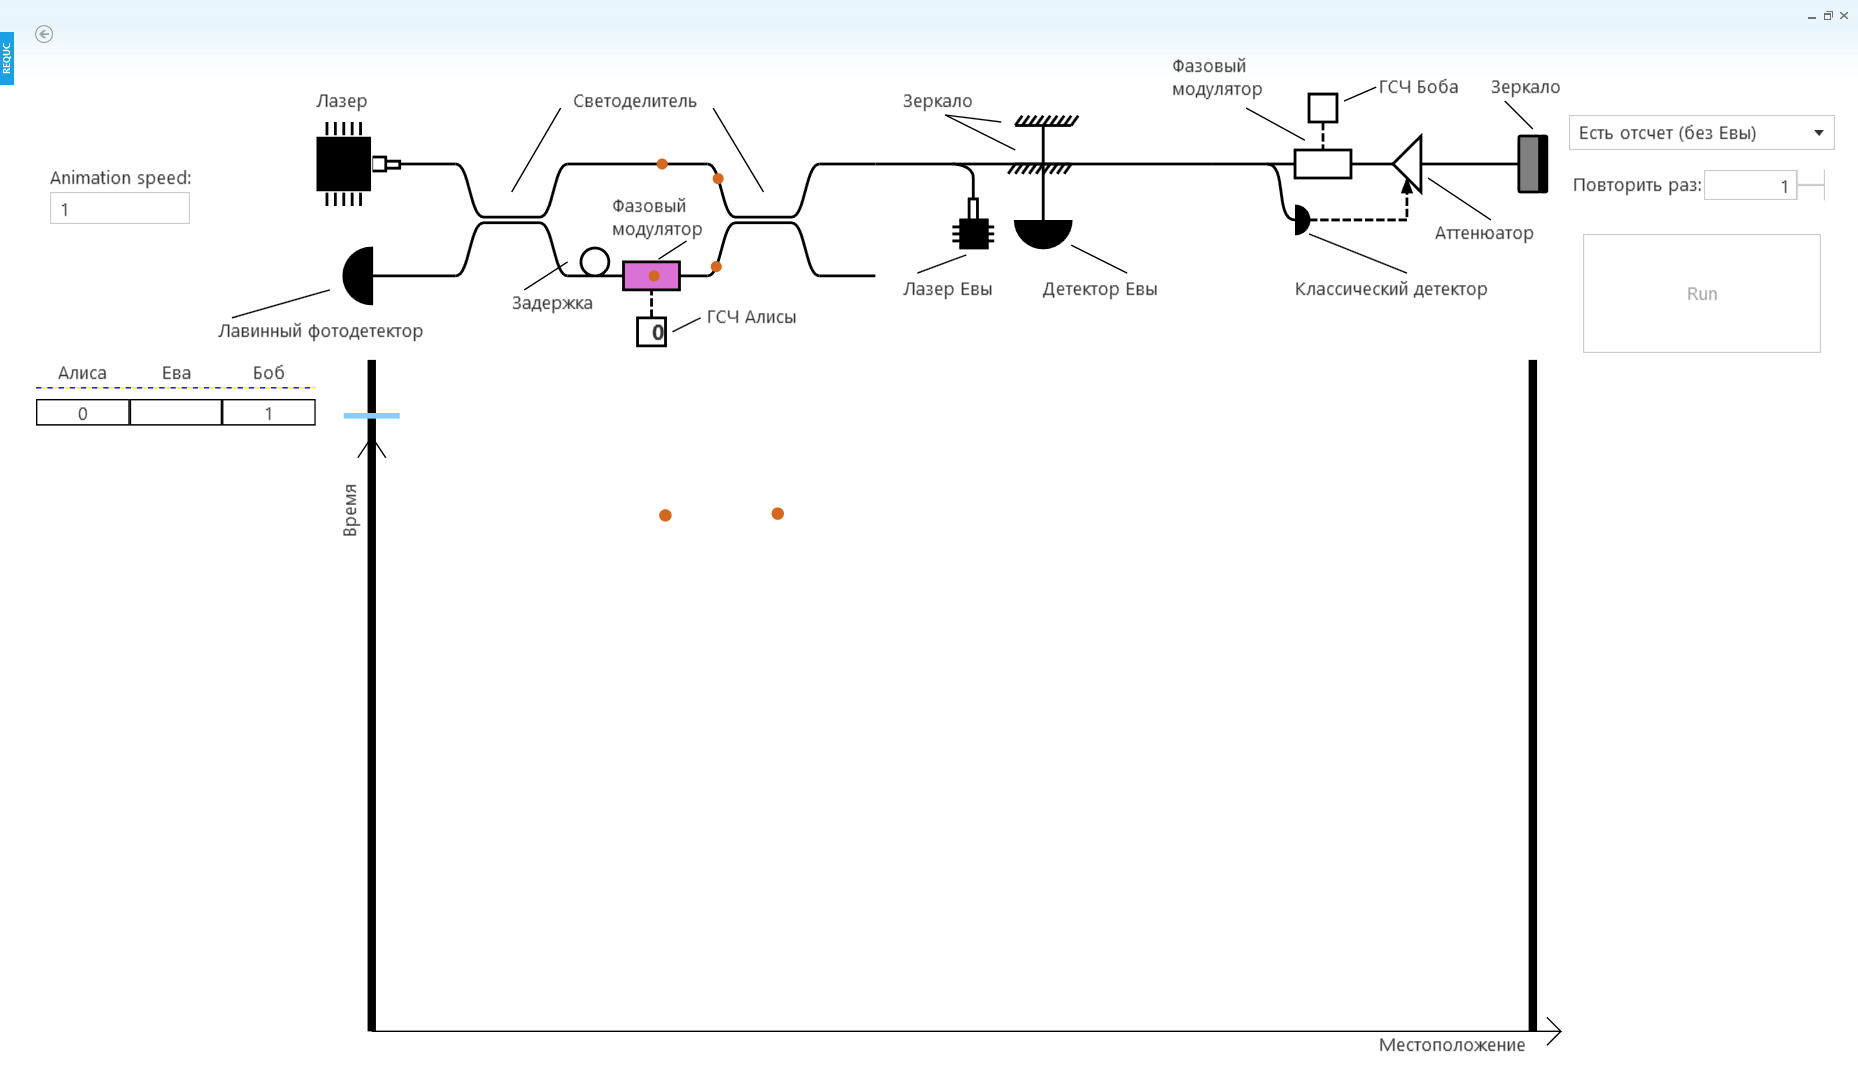
\includegraphics[width=0.9\linewidth]{chapter3/requc_screenshots/11_alice_phase}
  \caption{Алиса применяет фазовый модулятор к половинке состояния, локализованной в первом временном окне.}
\end{figure}

\begin{figure}[h]
  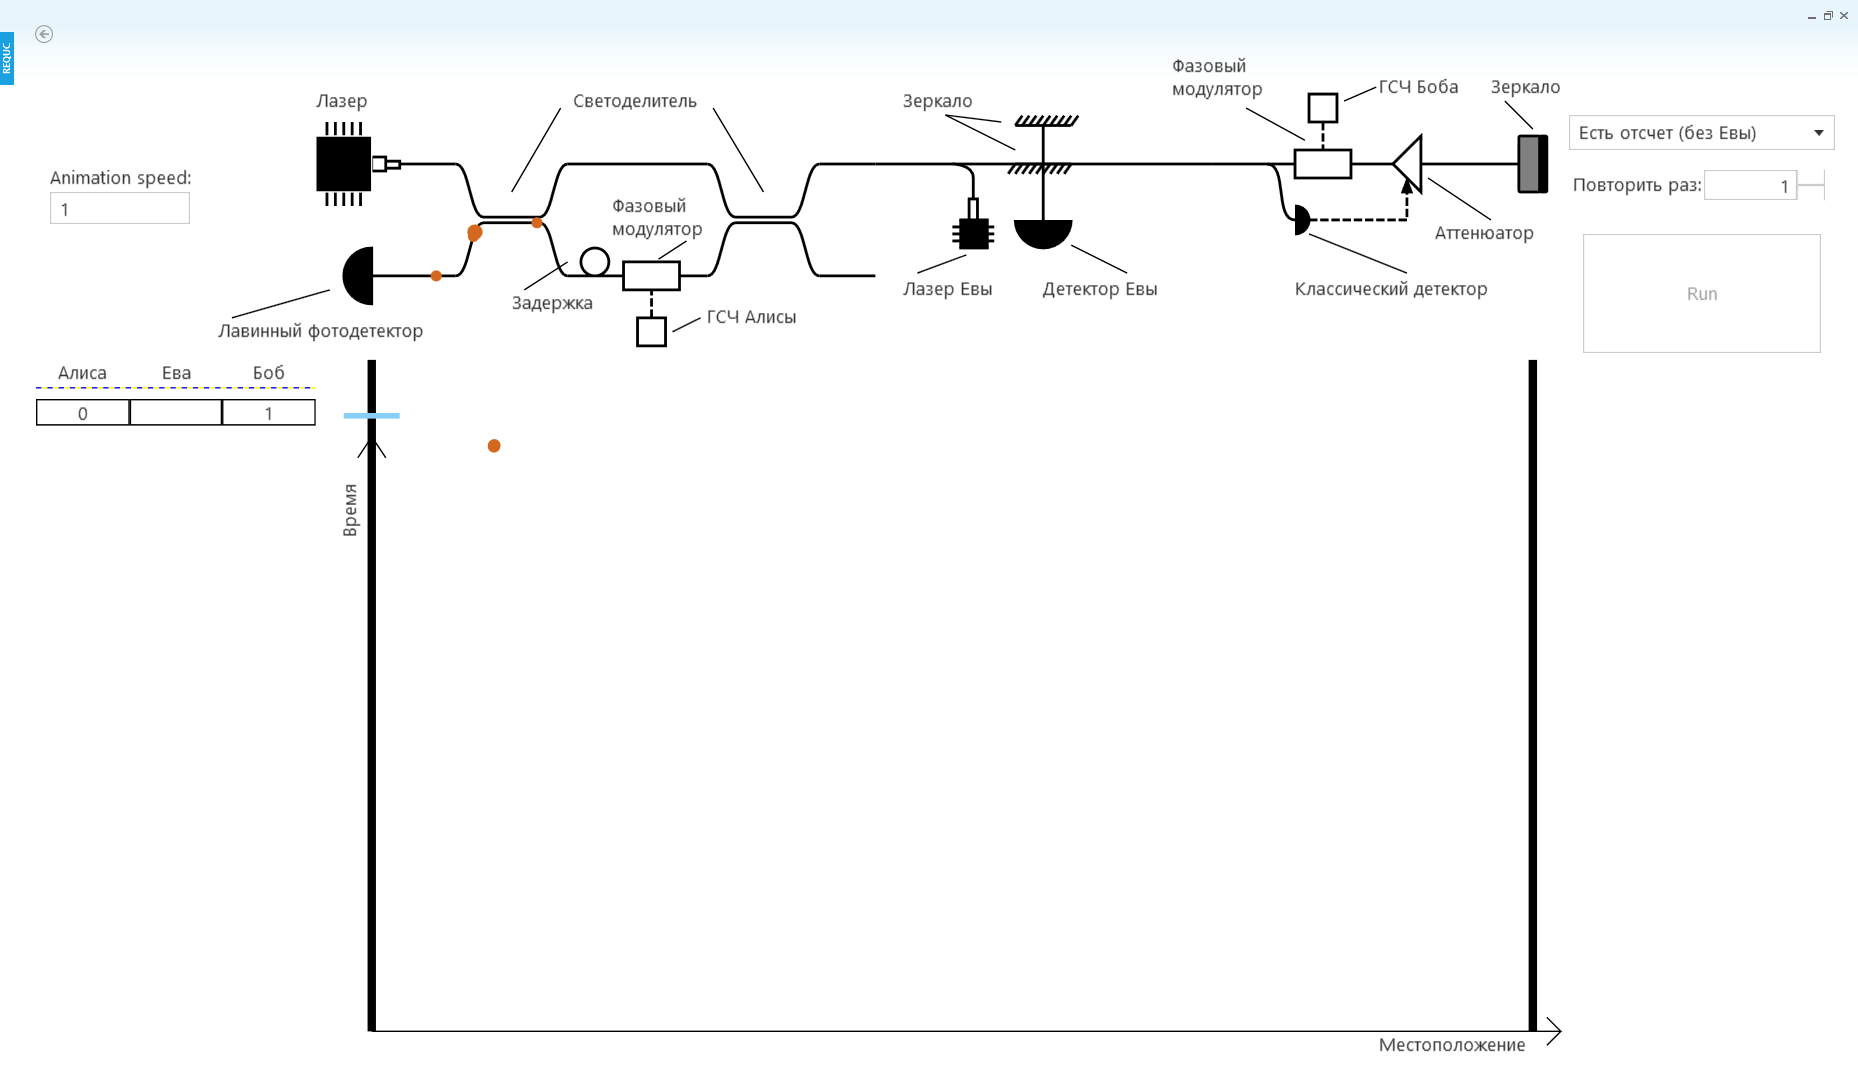
\includegraphics[width=0.9\linewidth]{chapter3/requc_screenshots/12_positive_interference}
  \caption{При выборе разных фаз Алисой и Бобом и последующем слиянии половинок на светоделителе происходит интерференция сигналов.}
\end{figure}

\begin{figure}[h]
  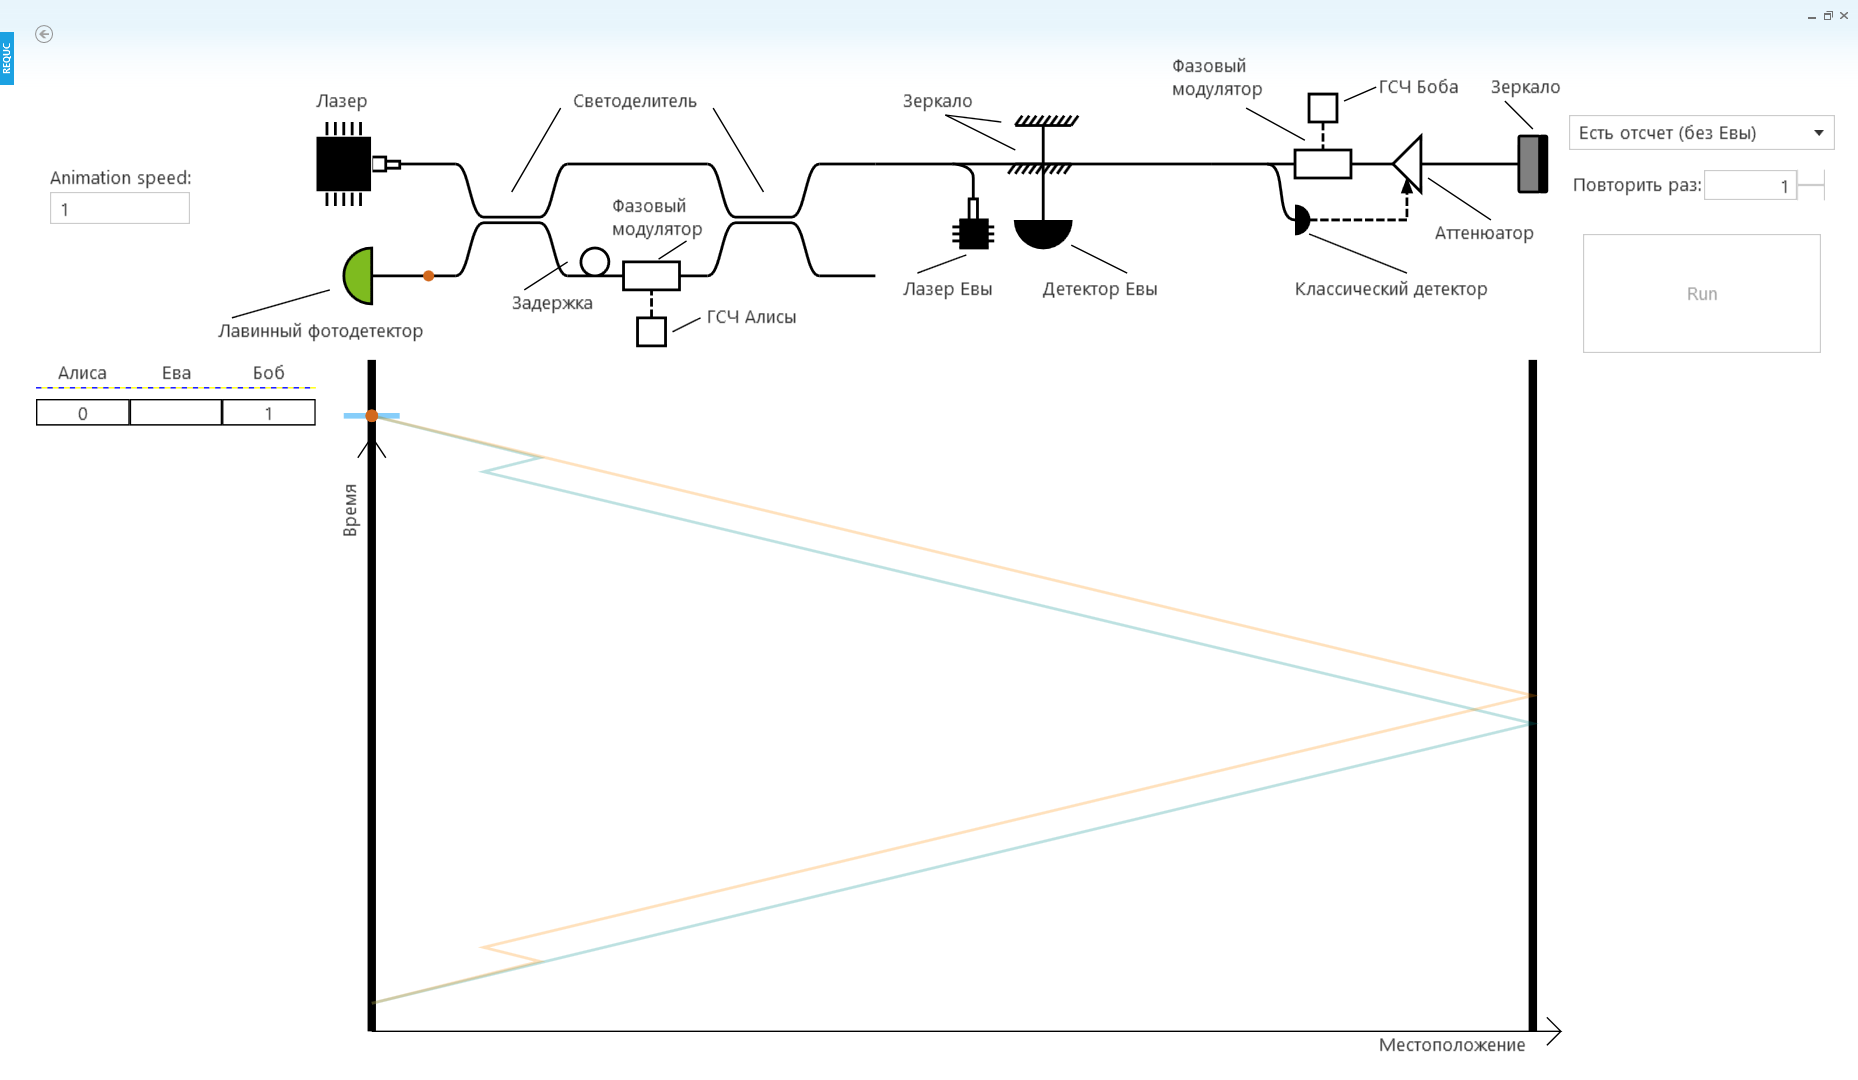
\includegraphics[width=0.9\linewidth]{chapter3/requc_screenshots/13_alice_detector}
  \caption{Отсчет детектора Алисы, свидетельствующий о том, что процесс завершился нормально, и сгенерированный бит войдет в ключ.}
\end{figure}

\begin{figure}[h]
  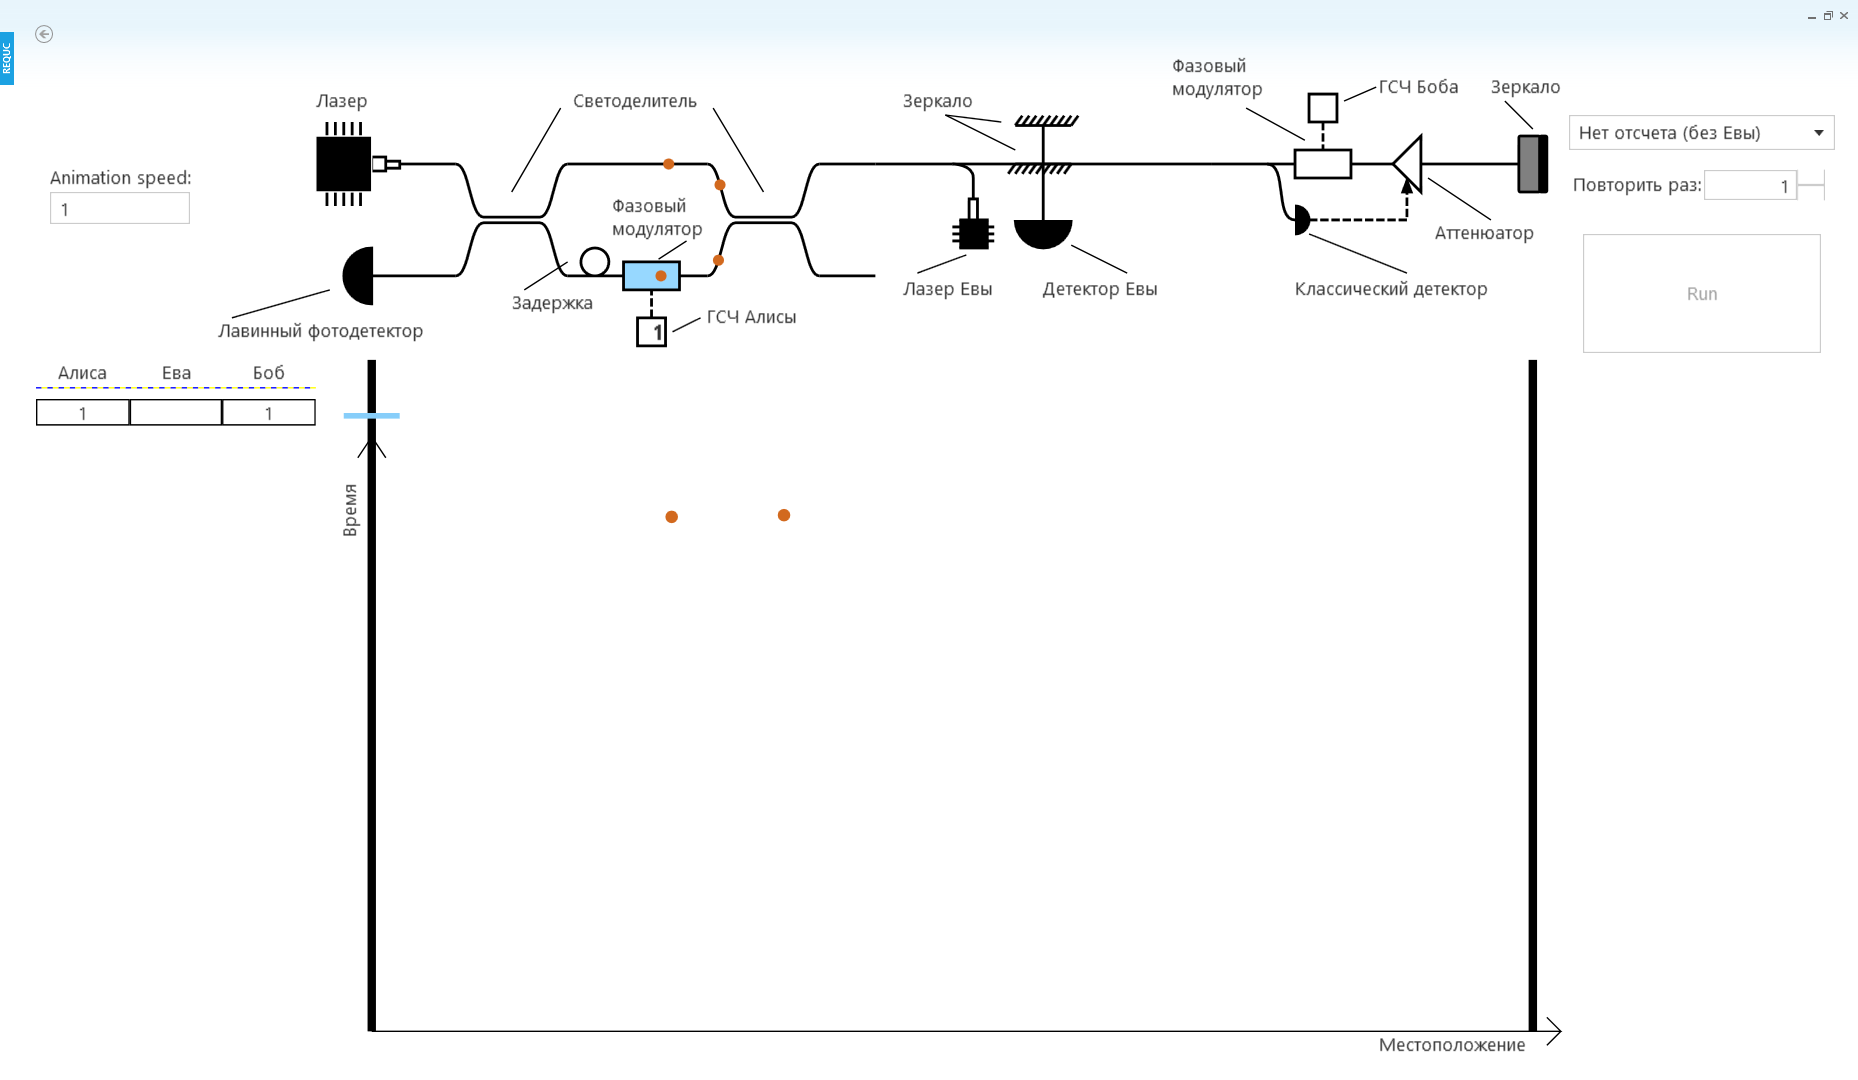
\includegraphics[width=0.9\linewidth]{chapter3/requc_screenshots/14_alice_phase}
  \caption{Алиса выбирает ту же фазу, что и Боб.}
\end{figure}

\begin{figure}[h]
  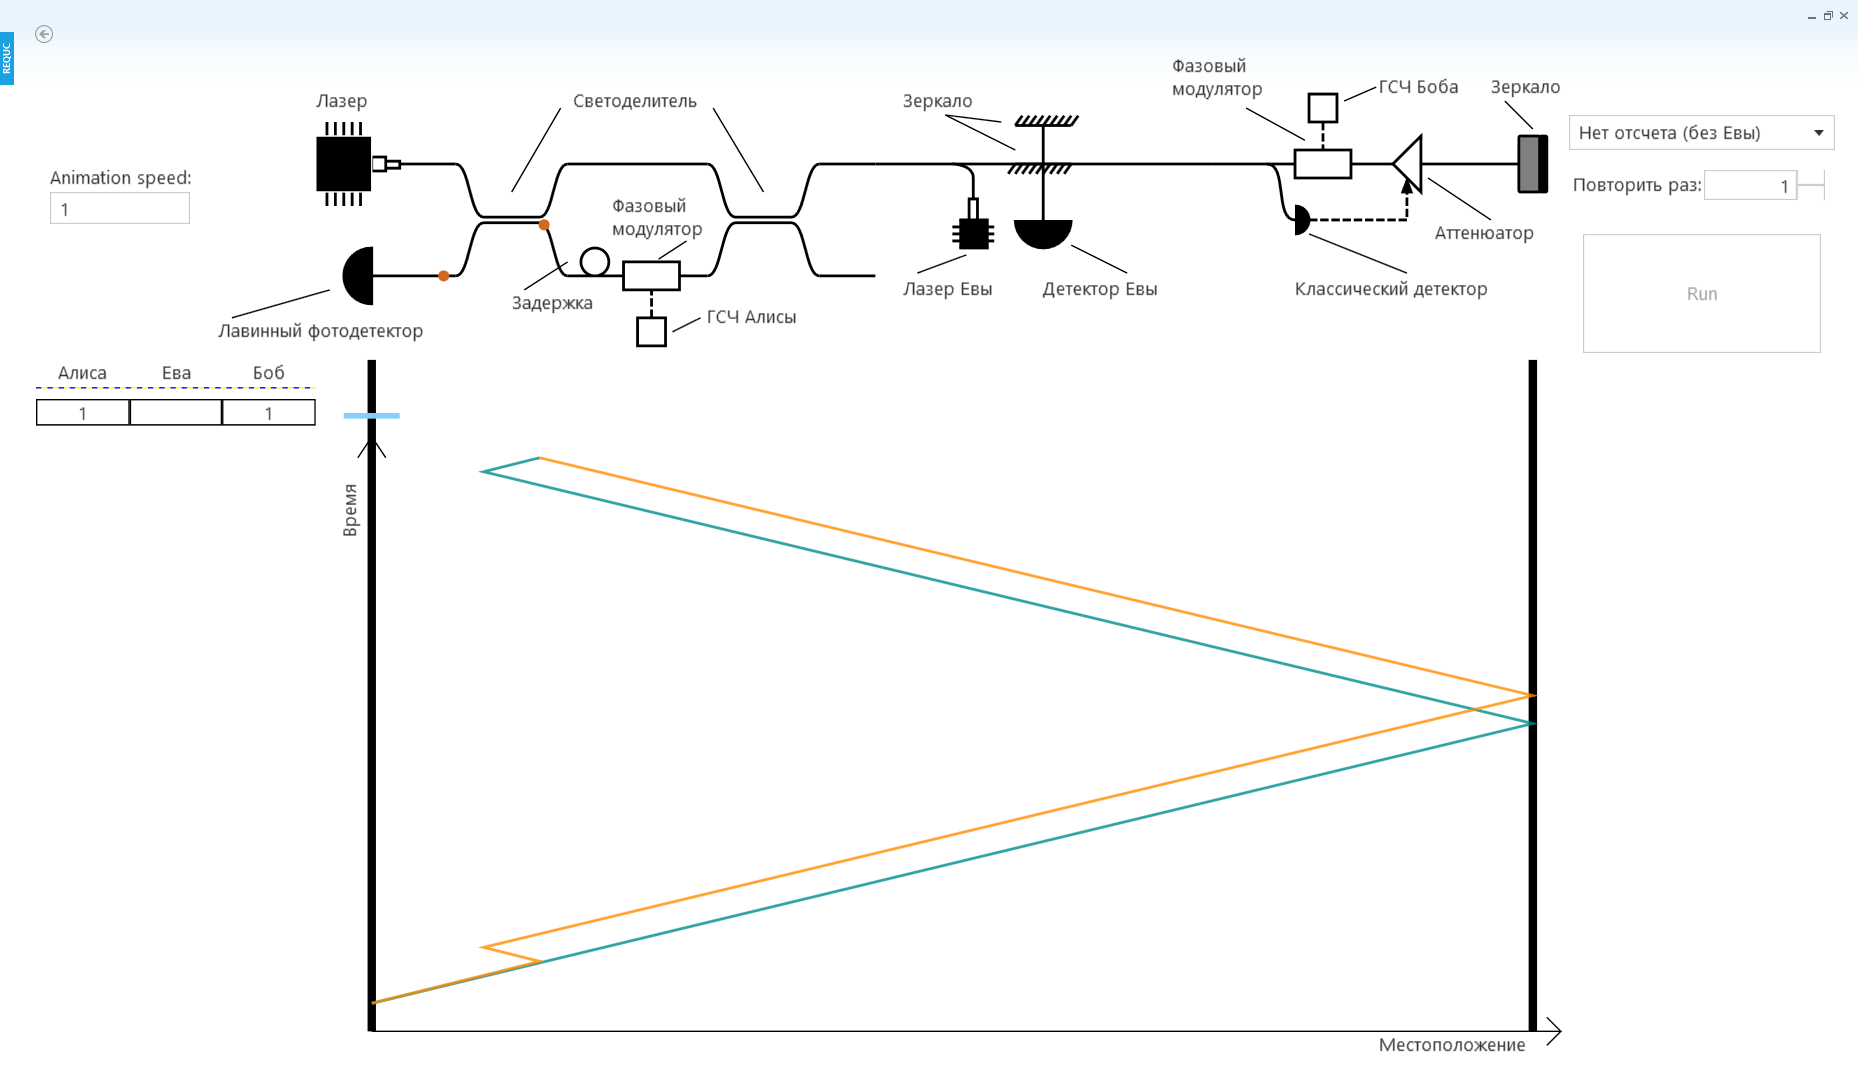
\includegraphics[width=0.9\linewidth]{chapter3/requc_screenshots/16_destructive_interference_2}
  \caption{Происходит деструктивная интерференция половинок, и в нужный временной интервал в детектор ничего не попадает.}
\end{figure}


\begin{figure}[h]
  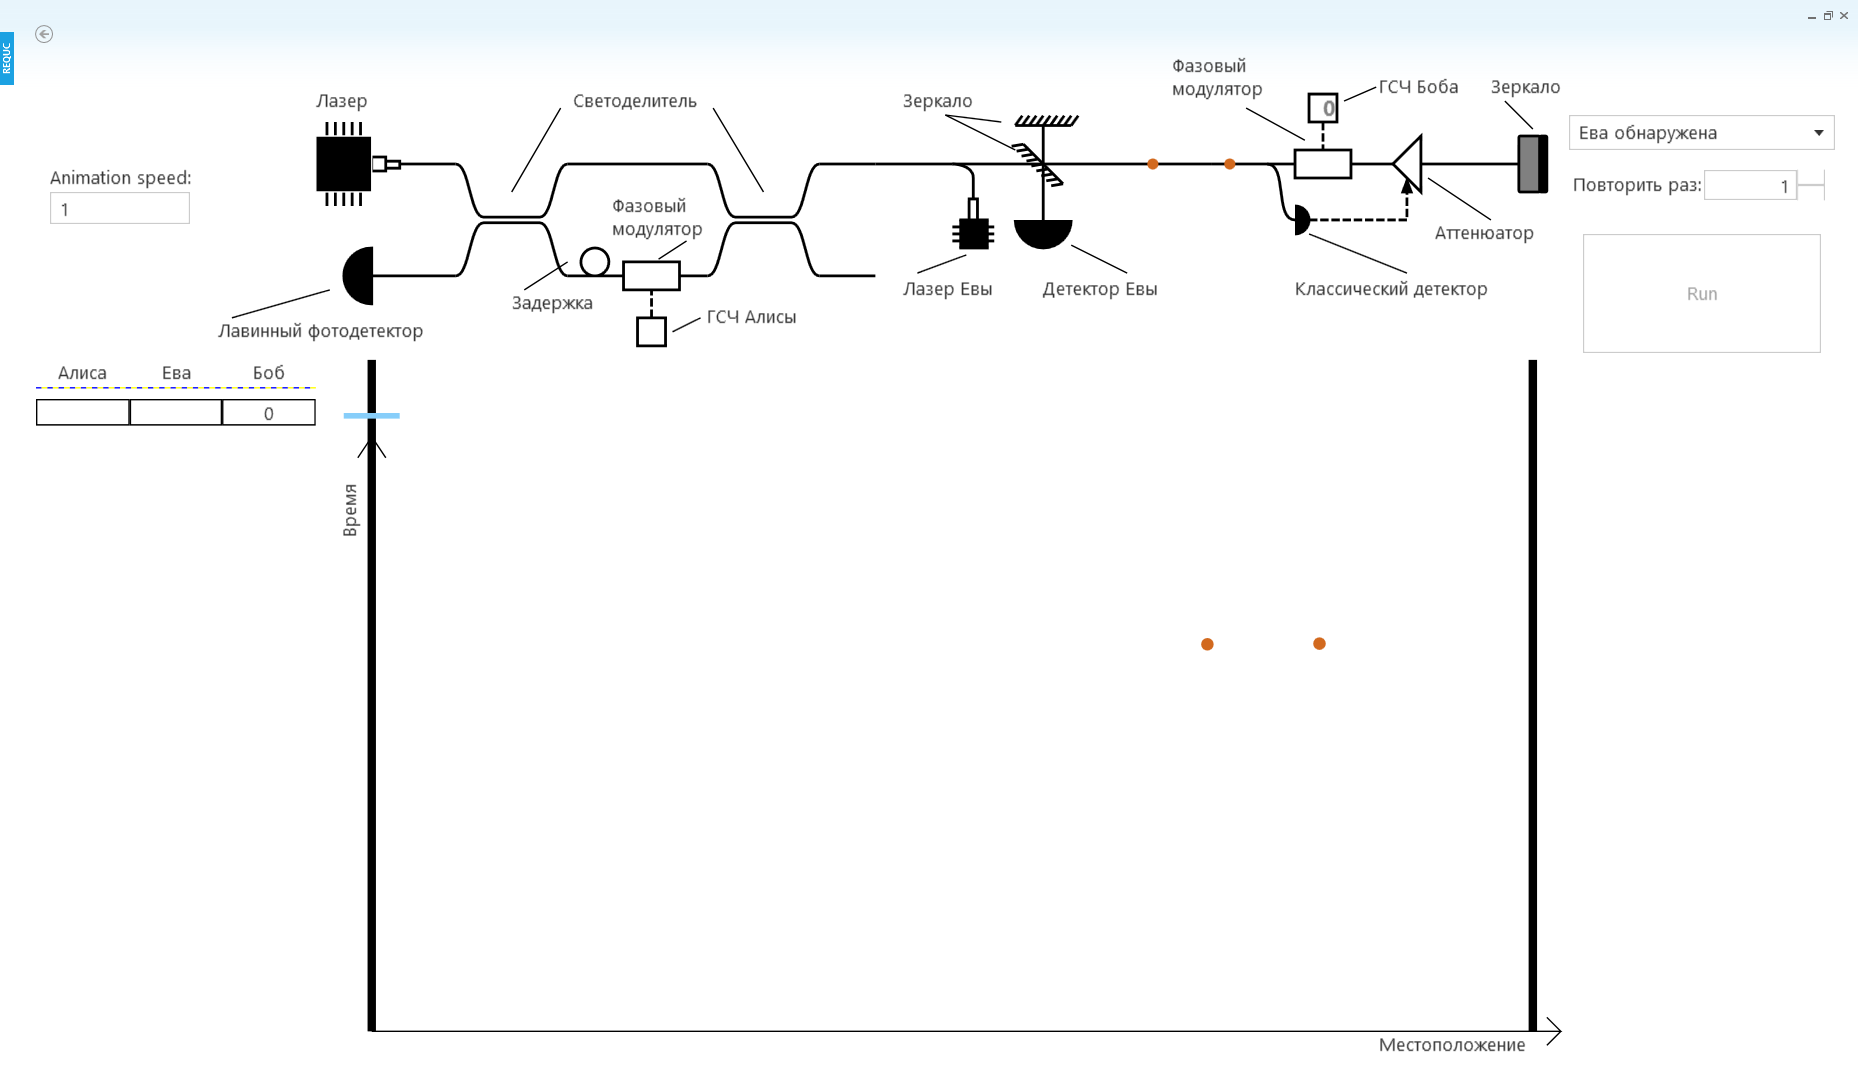
\includegraphics[width=0.9\linewidth]{chapter3/requc_screenshots/17_eva_catched}
  \caption{Ева решает перехватить посылку и выставляет зеркало на пути фотонов.}
\end{figure}

\begin{figure}[h]
  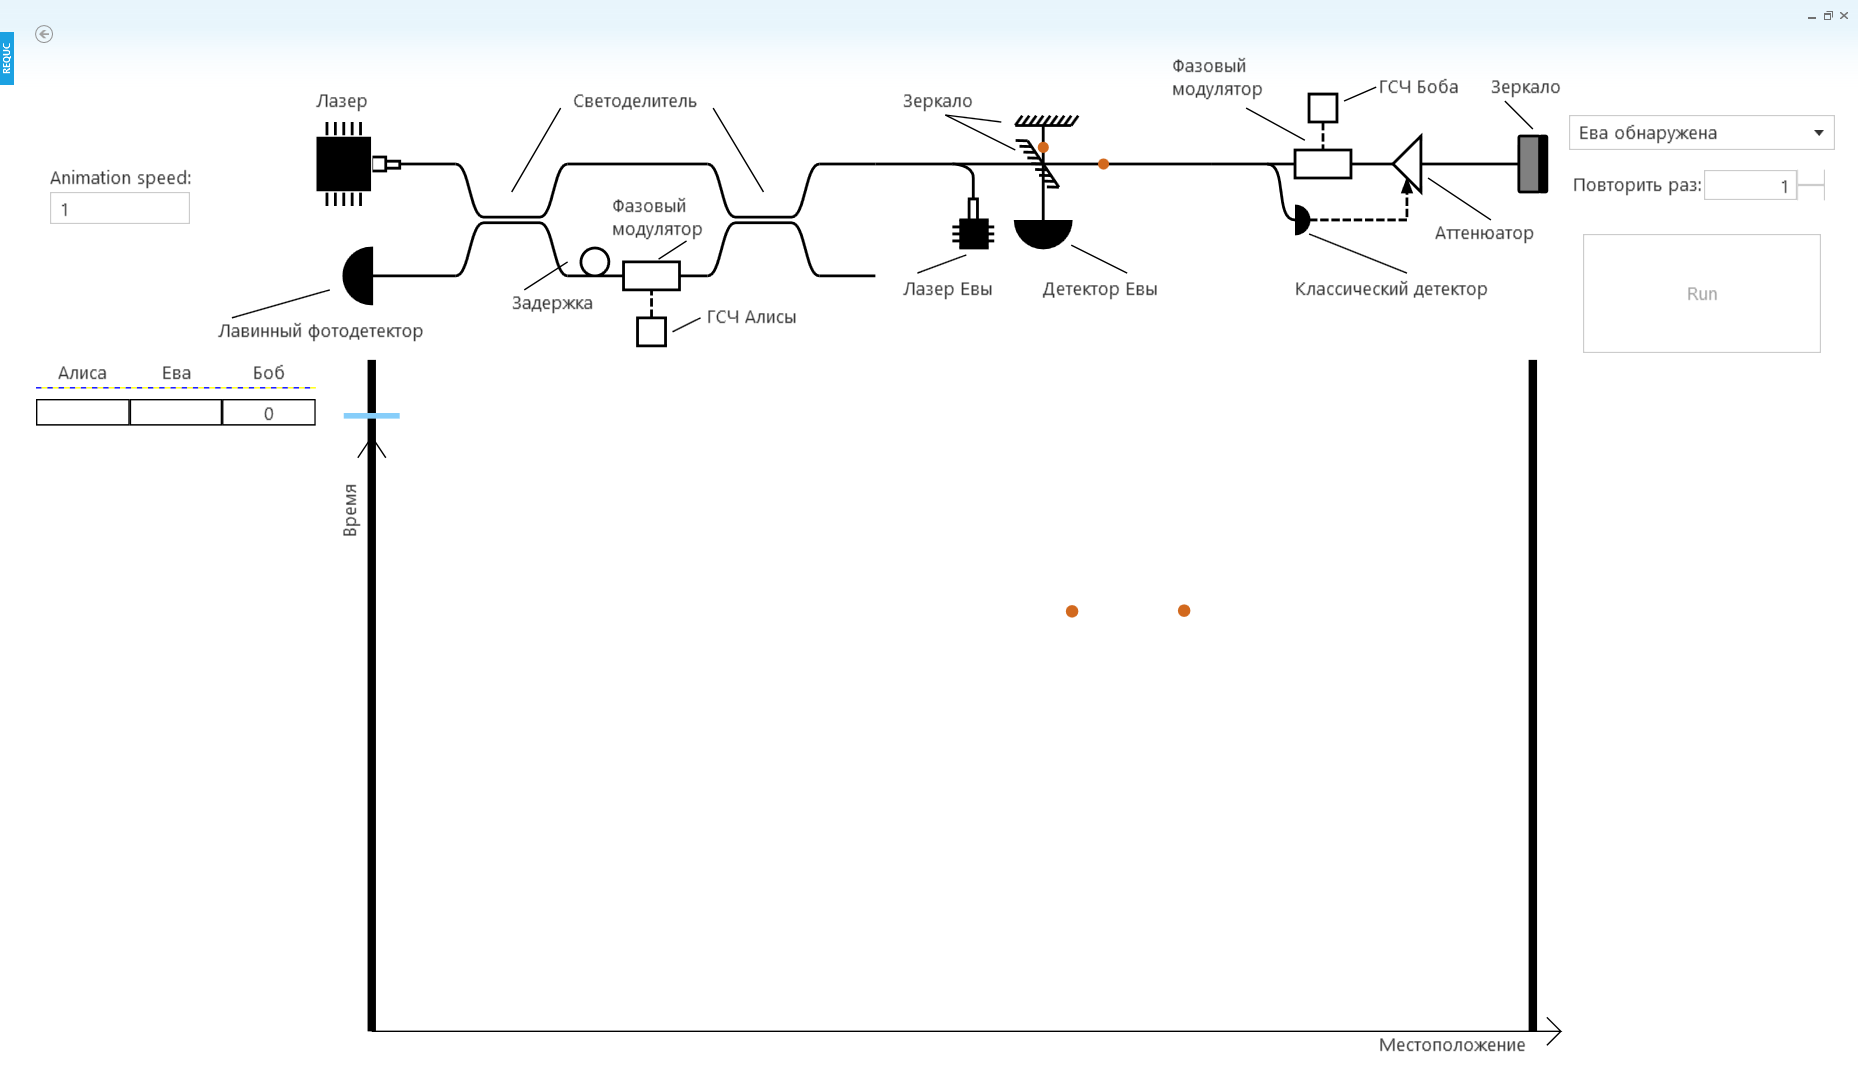
\includegraphics[width=0.9\linewidth]{chapter3/requc_screenshots/18_eva_mirror}
  \caption{Для сведения фотонов вместе требуется некоторое время, поэтому первая половинка совершает путешествие туда-обратно, пока до Евы не дойдет вторая половинка.}
\end{figure}

\begin{figure}[h]
  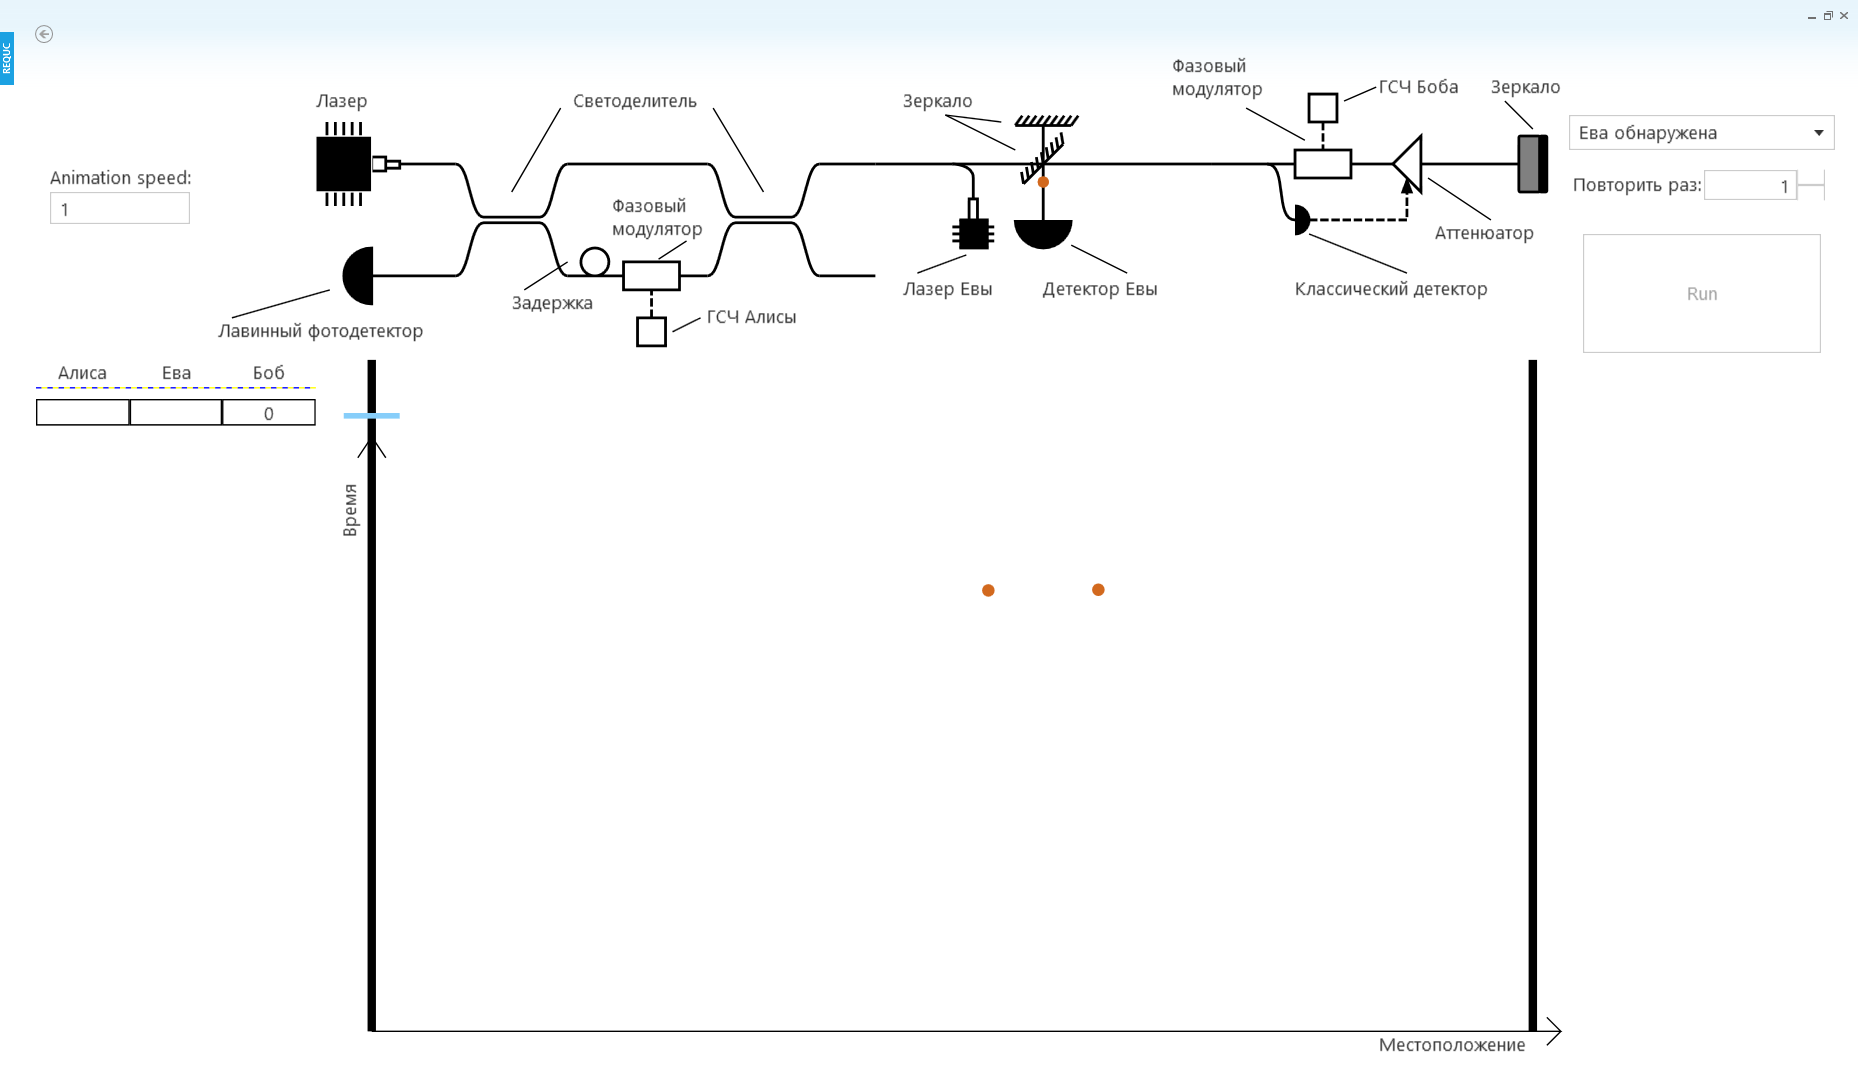
\includegraphics[width=0.9\linewidth]{chapter3/requc_screenshots/19_eva_detector}
  \caption{Половинки сведены вместе, теперь состояние можно отправлять в детектор.}
\end{figure}

\begin{figure}[h]
  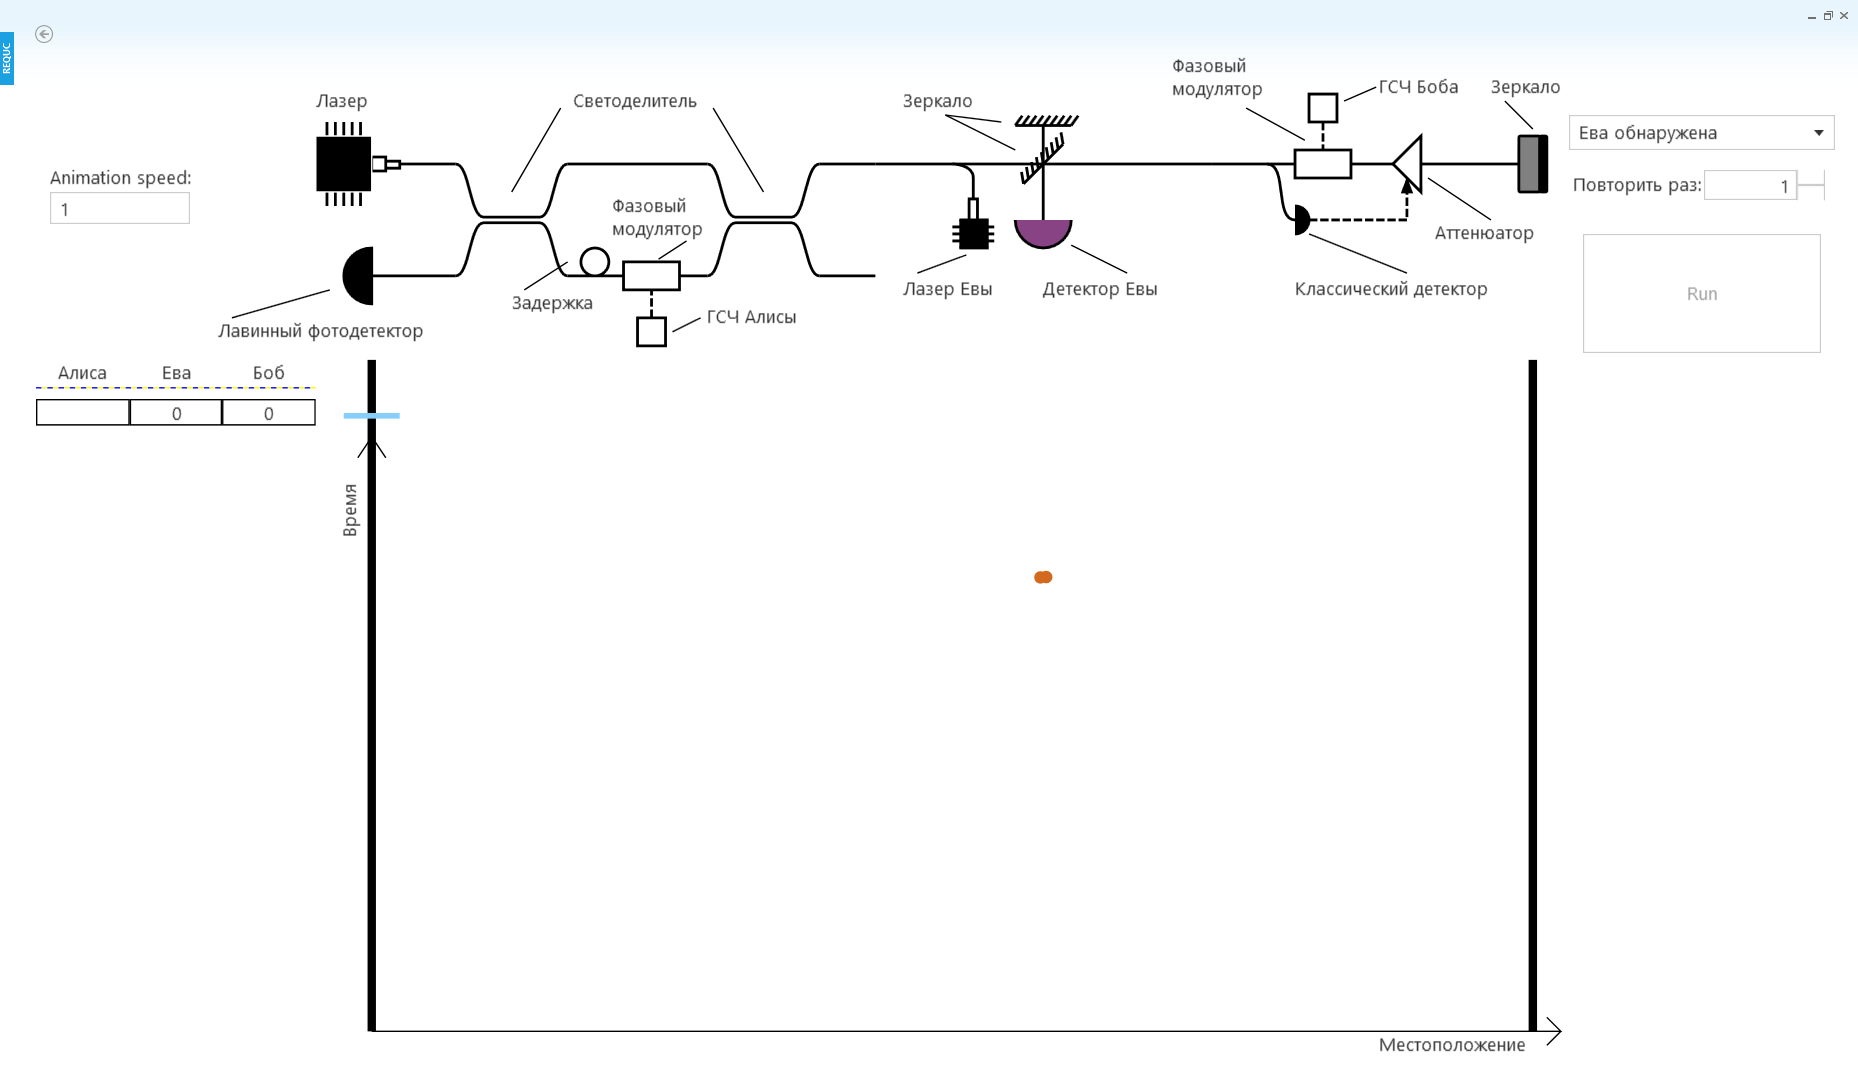
\includegraphics[width=0.9\linewidth]{chapter3/requc_screenshots/20_eva_measured}
  \caption{Проводится измерение с тремя исходами. В случае неопределенного исхода посылка блокируется.}
\end{figure}

\begin{figure}[h]
  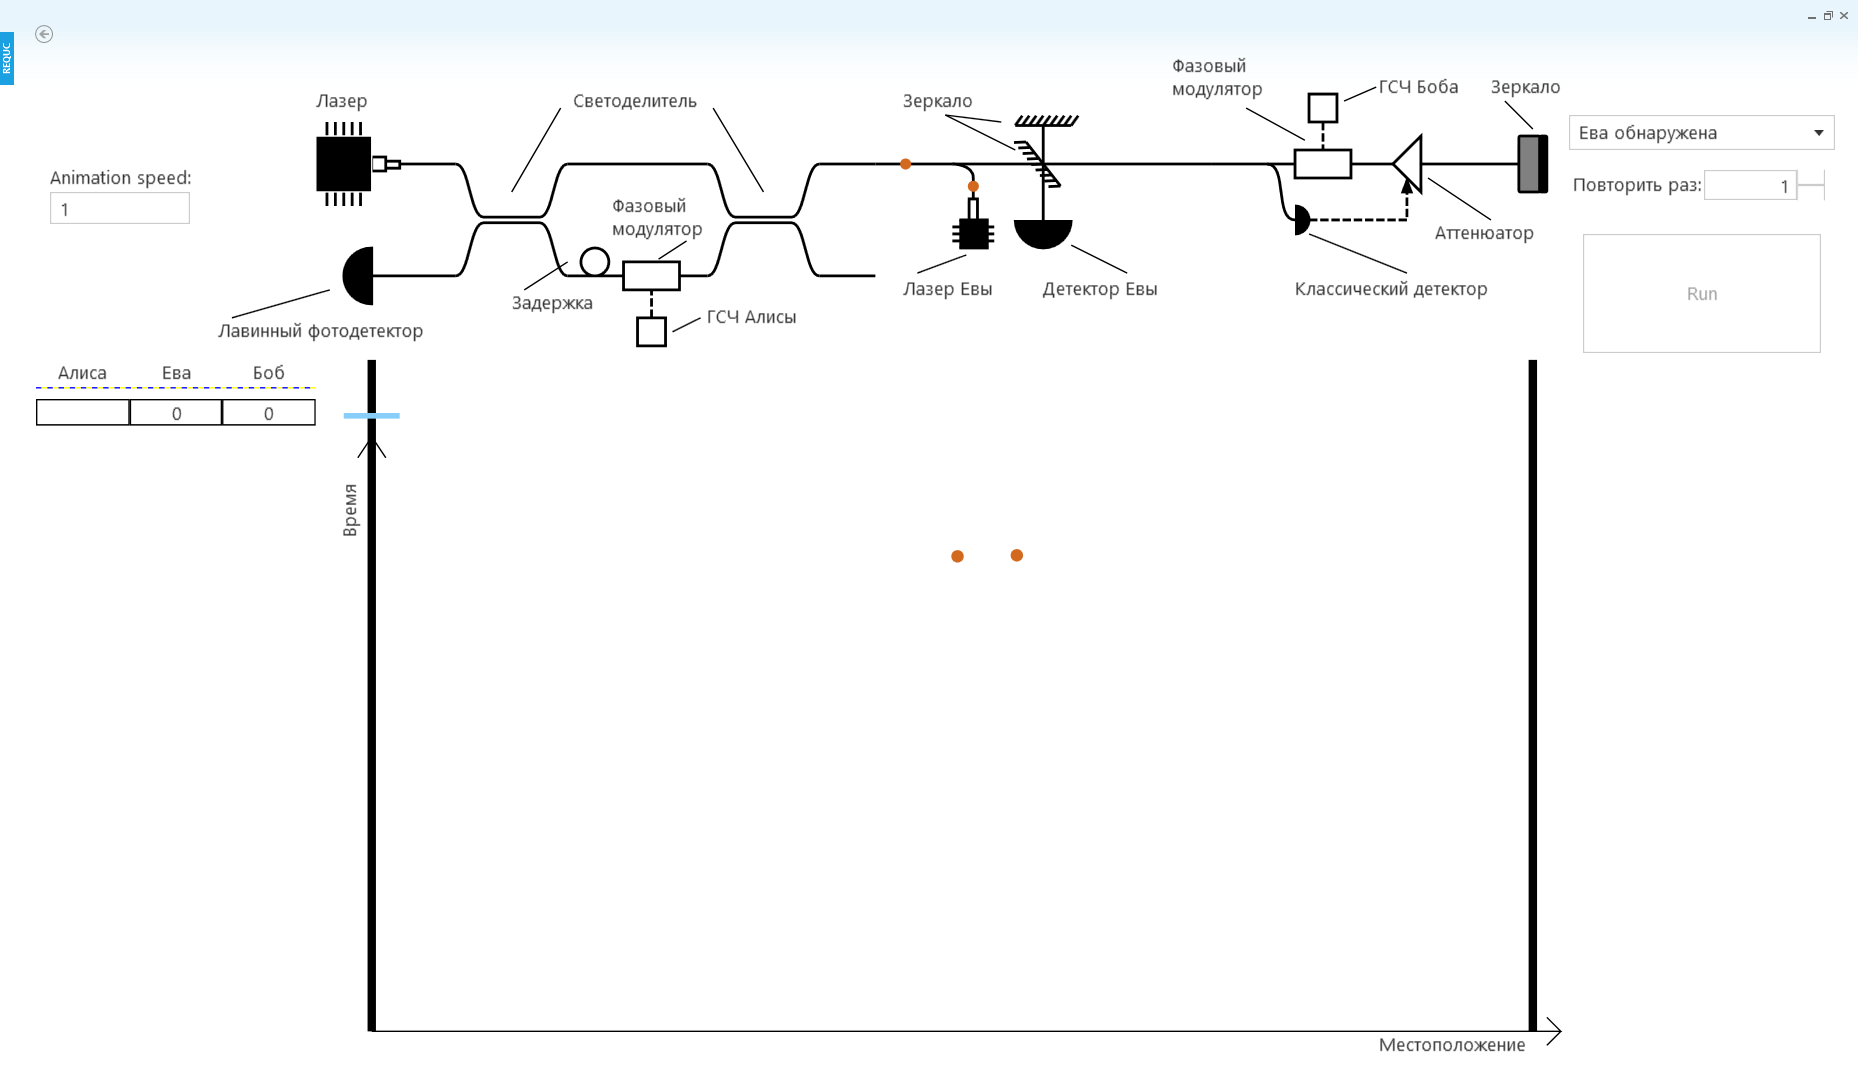
\includegraphics[width=0.9\linewidth]{chapter3/requc_screenshots/21_eva_laser}
  \caption{В случае определенного исхода Ева готовит такое же протяженное состояние, какое посылал Боб, и отправляет его дальше в канал.}
\end{figure}

\begin{figure}[h]
  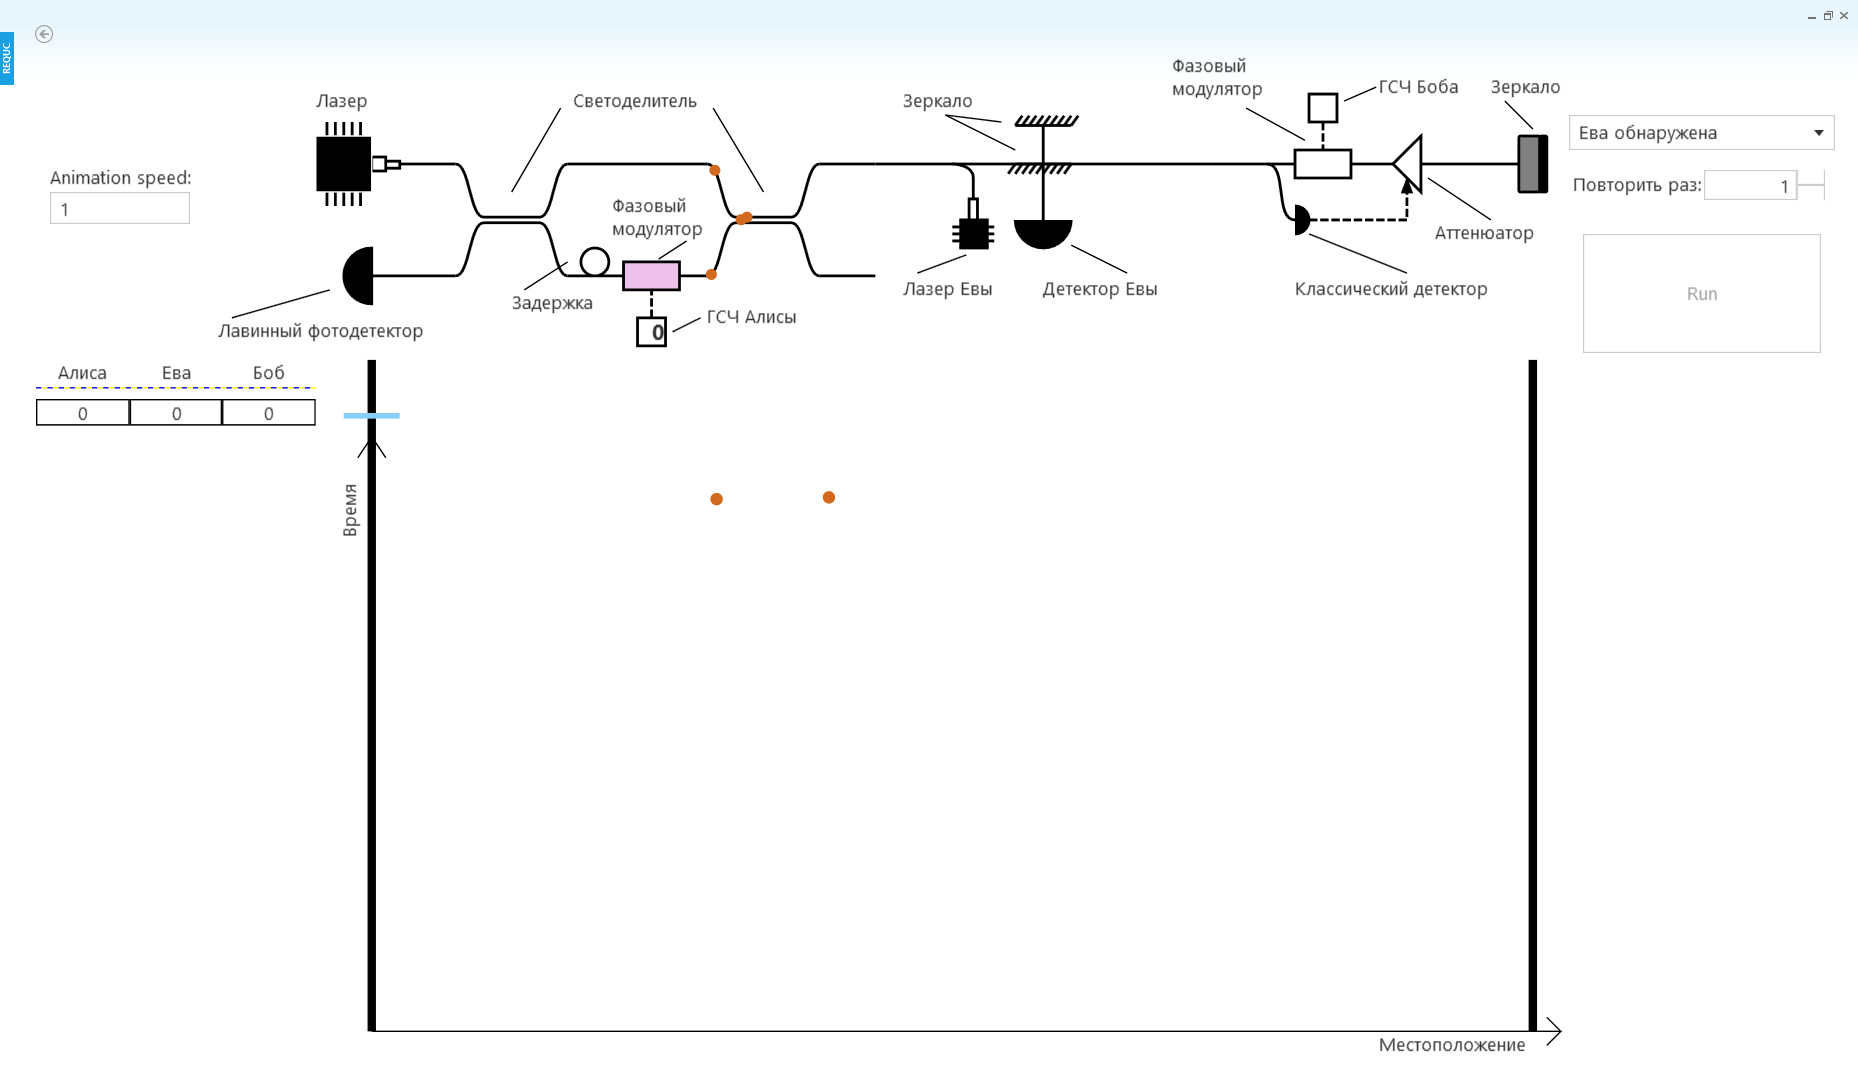
\includegraphics[width=0.9\linewidth]{chapter3/requc_screenshots/22_alice_phase}
  \caption{Из-за манипуляций Евы фазовый модулятор Алисы не применится к нужной половинке состояния, так как та не придет вовремя.}
\end{figure}

\begin{figure}[h]
  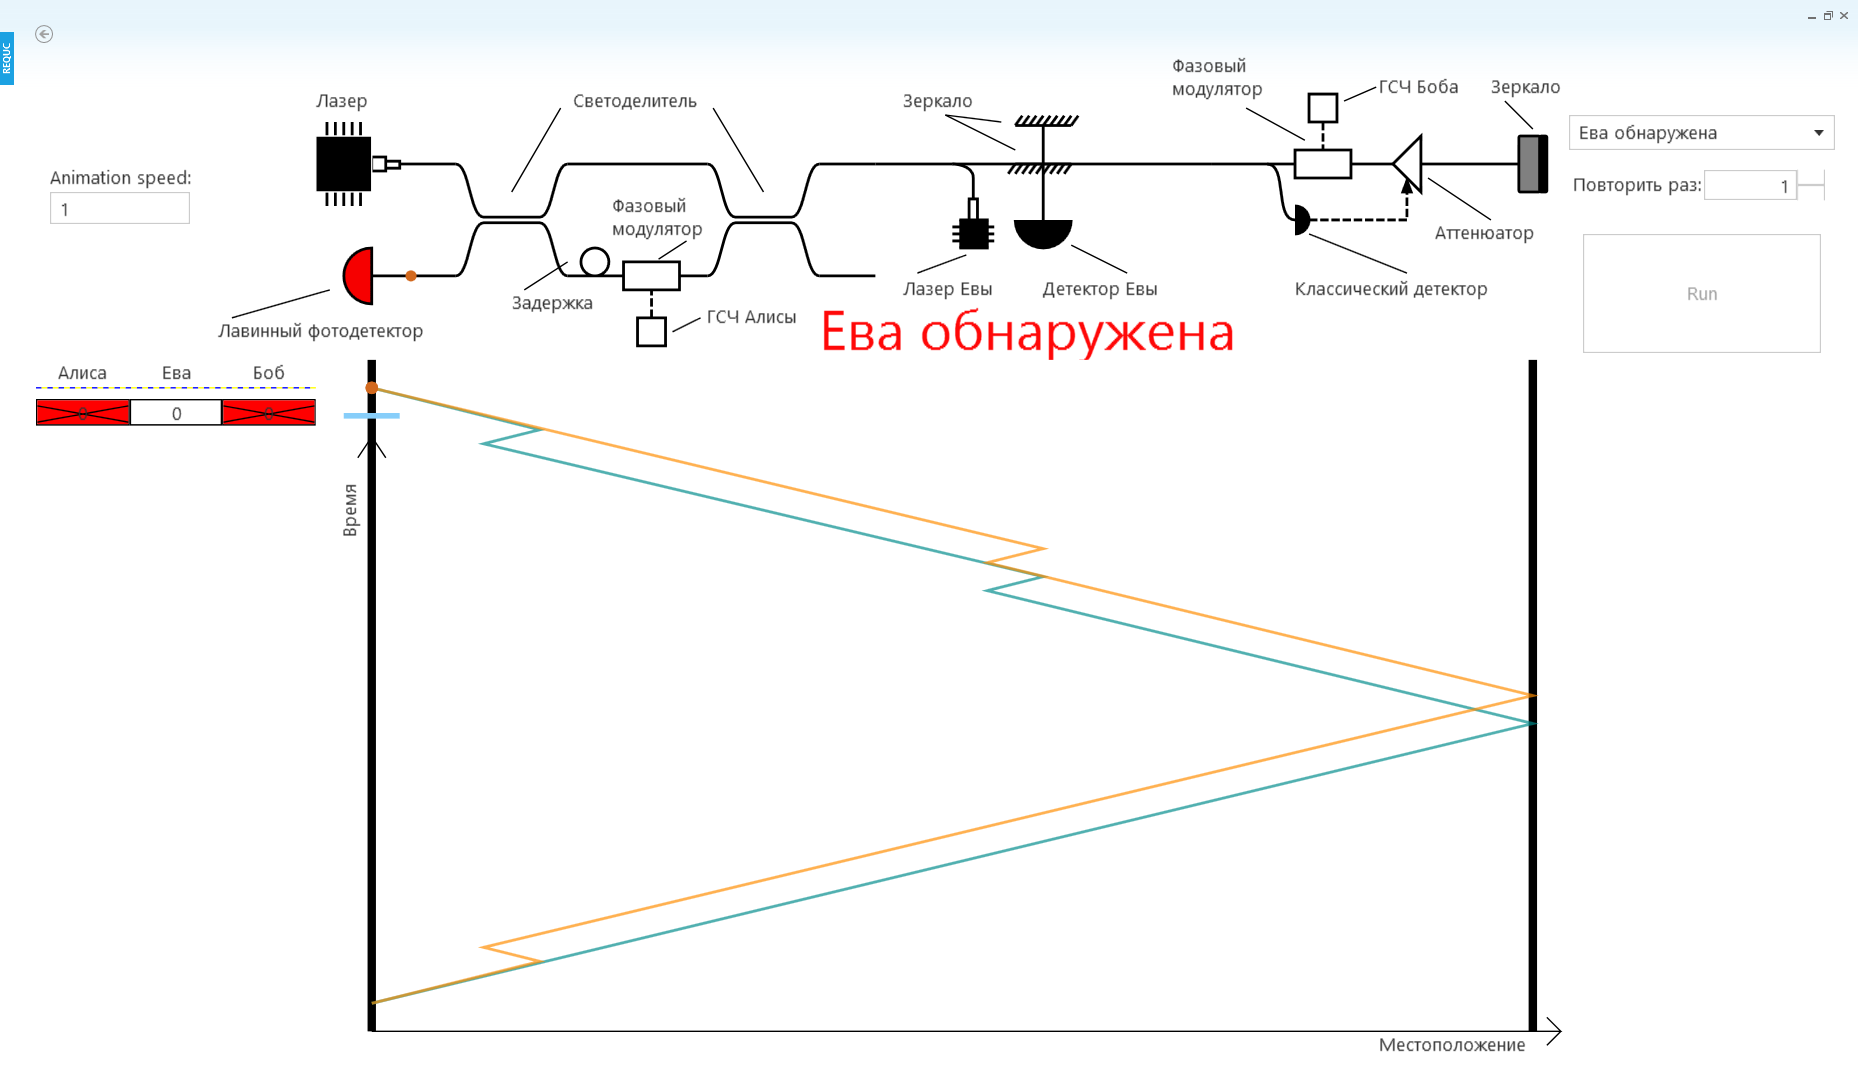
\includegraphics[width=0.9\linewidth]{chapter3/requc_screenshots/23_eva_detected}
  \caption{Фиксируется задержка состояния по времени, из чего делается заключение об имевшем место факте подслушивания. Соответствующие биты в ключ не войдут.}
\end{figure}

\FloatBarrier